\documentclass[10pt]{article}
\usepackage[letterpaper,margin=0.72in,top=0.65in,bottom=0.7in]{geometry}
\usepackage{amsmath,amssymb,amsfonts,mathtools}
\usepackage{booktabs}
\usepackage{longtable}
\usepackage{array}
\usepackage{tikz}
\usepackage{tikz-cd}
\usetikzlibrary{arrows.meta,decorations.pathreplacing,positioning}
\definecolor{ratered}{RGB}{176,36,40}
\definecolor{accblue}{RGB}{28,84,150}
\definecolor{compurple}{RGB}{110,50,140}
\usepackage[hidelinks]{hyperref}

\newcommand{\sJ}{\mathsf{J}}
\newcommand{\afrac}{\alpha_{\mathrm{frac}}}
\newcommand{\tr}{\operatorname{tr}}
\newcommand{\adj}{\operatorname{adj}}
\newcommand{\Path}{\mathsf{Path}}
\newcommand{\hbareff}{\hbar_{\mathrm{eff}}}
\DeclareMathOperator{\Real}{Re}
\DeclareMathOperator{\Imag}{Im}
\DeclareMathOperator{\spanop}{span}

\setlength{\parskip}{0pt}
\usepackage{titlesec}
\titlespacing*{\section}{0pt}{1.6ex plus .4ex minus .2ex}{0.8ex}
\titlespacing*{\subsection}{0pt}{1.2ex plus .3ex minus .2ex}{0.6ex}
\titlespacing*{\subsubsection}{0pt}{1ex plus .2ex minus .2ex}{0.5ex}
\setlength{\abovedisplayskip}{5pt plus 2pt minus 2pt}
\setlength{\belowdisplayskip}{5pt plus 2pt minus 2pt}
\AtBeginDocument{\setlength{\abovedisplayskip}{5pt plus 2pt minus 2pt}\setlength{\belowdisplayskip}{5pt plus 2pt minus 2pt}\setlength{\abovedisplayshortskip}{2pt}\setlength{\belowdisplayshortskip}{3pt}}

\newenvironment{symtab}[1]{\par\smallskip\fontsize{8.5}{9.8}\selectfont\renewcommand{\arraystretch}{0.88}%
\setlength{\LTpre}{0pt}\setlength{\LTpost}{0pt}\setlength{\LTleft}{0pt}\setlength{\LTright}{0pt}%
\begin{longtable}{@{}>{$}l<{$}p{0.37\textwidth}p{0.31\textwidth}l@{}}
\multicolumn{4}{@{}l}{\normalsize\textit{Symbols introduced in #1.}}\\[2pt]\toprule
\text{Symbol} & Meaning & Type & Ref.\\\midrule\endfirsthead
\toprule\text{Symbol} & Meaning & Type & Ref.\\\midrule\endhead}{\bottomrule\end{longtable}\par\smallskip}

\newcommand{\Derived}{\noindent\textsc{[Derived]}\ }
\newcommand{\Proposed}{\noindent\textsc{[Proposed]}\ }

\begin{document}

\begin{center}
{\large\bfseries On Information Physics: From State Distinguishability to Causal Accumulation}\\[4pt]
Categorical Composition, Biquaternionic Source Currents, and Lorentzian Structure\\[6pt]
Samuel Leizerman\\[2pt]
{\small LIOR Research Initiative \quad \href{mailto:sleizerm@asu.edu}{sleizerm@asu.edu} \quad ORCID: \href{https://orcid.org/0009-0000-0133-2291}{0009-0000-0133-2291}}
\end{center}

\begin{abstract}
Human cognitive architecture mirrors the mathematics of this note because the human brain is an embedded physical transducer forged under the invariant laws of the environment it evolved to predict. Human cognition is an embodied physical subsystem of nature, and it has no Markovian closure; a physical universe containing an evolved, non-Markovian observer must be capable of expressing non-Markovian dynamics, which contain the Markovian ones as limits rather than excluding them. Markovian dynamics is therefore confined to two limits, forgetful and faithful. Finite capacity and the Landauer bound make physical memory lossy, neither faithful to every history nor forgetful of all of them, and we propose that fundamental evolution is globally non-injective, which leaves a closed system only the forgetful limit. We begin by defining information as the distinguishability of physical states and causality as change in physical state, including its rate of change. The fundamental theorem of calculus connects instantaneous change to accumulated change, but endpoint displacement alone does not retain a weighted causal history. Causal histories compose, motivating a path-category description; comparison of contributions at different spacetime points additionally requires transport. The de Rham complex places endpoint dependence, topological path dependence, and curvature on three tiers, and situates the history functional outside all of them. We then construct the source algebra, which yields two finite-dimensional constructions: positive biquaternionic closure with Born-rule trace readout, and Lorentzian determinant geometry on the same matrix carrier. The real forms of that determinant separate the Hermitian closure slice, which carries Minkowski four-vectors, from the anti-Hermitian generator slice, on whose traceless part the determinant is proportional to the Killing form of $\mathfrak{su}(2)$, with factor $-\tfrac18$. Dyads of closure vectors give rank-two tensors that satisfy the weak, null and dominant energy conditions by positivity alone, and these conditions survive causal accumulation automatically for interaction depth $\afrac\ge1$. The proposed Causal Accumulation Law (CAL) then combines these ingredients in a past-supported integral. For an action weighted by a positive function, the gradient of the weight adds a friction-type term to the Euler--Lagrange equations; we derive this, and we derive the weight itself as accumulated causal weight by exchanging the two integrations of the history-weighted action, whose sign the law forces; finiteness of that weight remains open. A closing sketch states the cognitive-evolutionary hypothesis that motivates the program and the evidence that supports it. This note develops the foundational mathematical structure from which the full field dynamics are intended to be mapped. The construction of those dynamics is an active research effort, not a result asserted here; further field equations, dynamical regimes, and gravitational extensions fall beyond the present scope.
\end{abstract}

\section*{Introduction}

Human cognitive architecture mirrors this mathematics because the human brain is an embedded physical transducer forged under the invariant laws of the environment it evolved to predict. If an organism's internal world-model violates the geometric and causal constraints of the physical medium it navigates, it miscalculates trajectories, misallocates metabolic energy, and dies. Human evolution did not construct an arbitrary symbolic computer; it tuned neural mechanics to be homomorphic to physical reality.

\smallskip
\noindent\textbf{The kinematic window: why we perceive state as $[x,v]$.} In Sec.~1 the physical state is the two-slot container $X=[x,v]$, where acceleration $a=g(x,v)$ is fixed by the law and higher derivatives recurse back through the same vector field, $TQ\to T^2Q$. Nature closes its dynamical laws at second order; third-order laws carry runaway solutions and instabilities (Ostrogradsky, Abraham--Lorentz). The human sensory-motor apparatus is tuned to this boundary. The vestibular system does not measure jerk or higher derivatives directly: the otolith organs sense linear acceleration, the semicircular canals sense angular motion, and linear velocity is obtained by accumulating acceleration over time~\cite{angelaki}. Visual cortex (area MT/V5) dedicates large neural populations to optical flow and velocity. We track position and velocity as a unified perceptual state $[x,v]$ because that is the jet bundle where physical mechanics closes.

\smallskip
\noindent\textbf{Metabolic limits and fractional memory.} A biological brain operates on an extreme thermodynamic budget, roughly 20 watts, and faces a trade-off between two unviable extremes. The Markovian limit is purely reactive, memoryless behavior. In Eq.~\eqref{e:9} it is reached in two ways: at $\afrac=1$, where the history term vanishes for every kernel, and at any $\afrac$ when the kernel concentrates at the present, $k\to\delta$. At $\afrac=0$ the $\delta$-kernel gives Newton's first law, while the same depth with a light-cone-supported kernel gives the opposite extreme, the relaxed Einstein equations in harmonic gauge, whose post-Minkowskian solution is a delayed integral supported on the past light cone. An animal that cannot retain past trajectory history cannot anticipate predatory pursuit, track seasonal prey migrations, or infer causal agency. The jet-expansion limit, storing an ever-expanding stack of discrete past states or higher-order derivatives, requires unbounded memory registers and amplifies high-frequency sensory noise. Evolution's solution is power-law adaptation and fractional accumulation of the form of Eq.~\eqref{e:20}. Cortical spike-frequency adaptation and human memory decay follow power laws rather than simple exponentials~\cite{lundstrom,wixted}. Fractional accumulation gives the mind scale-free temporal memory: it retains long-range historical context without paying the metabolic and computational penalty of an exploding state space.

\smallskip
\noindent\textbf{The dual substrate: perception and deliberation.} The channel amplitude of Eq.~\eqref{e:10} binds two structures into one complex carrier, the decay sector $e^{-H_a/\tau_E}$ and the phase sector $e^{iS_a/\hbareff}$. Human cognition is split between two functional modes that map onto these terms. Perception and perceptual inference operate like a thermodynamic or Bayesian estimator, damping sensory noise through energy-minimizing statistical weights. Deliberation, counterfactual planning, and language do not behave like classical probabilities: human choice displays interference effects, context dependence, and strong order dependence~\cite{wangqo,busemeyer}. By housing both in $M_2(\mathbb C)$, the left closure $\sJ\sJ^\dagger$ is a positive state readout that preserves non-commutative sequence order, $J_{tx}J_{tx}^\dagger\neq J_{xt}J_{xt}^\dagger$ (Eq.~\eqref{e:47}), while yielding normalized, positive probabilities through trace evaluation (Eqs.~\eqref{e:14}--\eqref{e:15}). Human cognition exhibits quantum-like decision algebra because an organism weighing alternative futures must model interference between counterfactual paths, not merely tally classical sums.

\smallskip
\noindent\textbf{The syllogism, C1--C5.} The argument of this note is a three-step syllogism.
\begin{description}\itemsep1pt
\item[C1, C2.] Information is physical. Cognition is information processing. Cognition is therefore physical: an embodied subsystem of nature.
\item[C3.] Cognition is non-Markovian. A snapshot of every neuron firing at instant $t$ does not determine the agent's intent or next action without the weighted historical context of how that state was reached. Cognition is a physical subsystem, and a subsystem is the image of its supersystem under a non-injective map (Sec.~2): a physical part, taken together with its couplings to the rest. Eliminating the rest from the equations, as with the coupled oscillators of Sec.~1, is also non-injective, but it produces a reduced representation, not a subsystem; the memory kernel of that representation comes from the elimination. The history dependence of cognition is a claim about the subsystem itself: given its full physical state and its inputs at time $t$, its next state is still not determined without its history. A property of the subsystem must therefore be expressible by the physical supersystem.
\item[C4, C5.] Markov models are the $\delta(\tau)$ limit. A physical universe containing an evolved, non-Markovian observer cannot be restricted to Markovian dynamics; physics must therefore be capable of expressing non-Markovian dynamics. This does not prohibit Markovian dynamics: a history-dependent law contains them as its limits, the kernel concentrating at the present or the history weight vanishing, whereas a Markovian law on the same variables cannot express history dependence without enlarging its state. Markovian dynamics is confined to two limits, forgetful and faithful (Sec.~1), and under the postulate of global non-injectivity proposed in Sec.~2 a closed system can reach only the first.
\end{description}
Human minds could only evolve non-Markovian causal reasoning in a universe that retains causal history along its past light cones $J^-(x)$. We model physical reality with ordered causal narratives because physical reality preserves ordered, transported causal history. Reality is neither faithful to every history nor forgetful of all of them (Sec.~2).

Human evolution did the heavy lifting by pruning every sensory, cognitive, and neural architecture that failed to track the invariants of spacetime. What feels like intuitive physics to a human, namely the directionality of time, the stability of second-order motion, the non-commutativity of actions, and the persistence of memory, is the structural imprint of the universe's algebraic constraints stamped into neural tissue. The sections below formalize that structure, and Sketch~4 of Sec.~7 collects the supporting evidence.

The hypothesis of this note is that physical law is history dependent, with the Markov models as its limits, and that the same structure underlies the history dependence of cognition. The Causal Accumulation Law comes from lifting causal inference~\cite{pearl} into a field theory and adding non-Markovian dynamics: causal structure becomes ordered transport on a causal past, and the influence of that past is accumulated rather than truncated to the present. The claim is not new physics but an assembly: established mathematical and physical structures, from the fundamental theorem of calculus to spinor geometry and causal transport, combine into one coherent construction.

The end goal is to replace the softmax query--key--value attention of transformer architectures~\cite{vaswani} with a field-theoretic vector interaction, one capable of bridging information interactions to the stress--energy tensor $T^{\mu\nu}$ and to the other structures a field theory requires. The falsifiability objective is white-boxed agent-based modeling: agents carrying an internal coordinate state in spacetime, so that agent-based models become stateful and non-Markovian, and evolutionary game theory~\cite{maynardsmith} can be run with history-dependent strategies whose predictions are open to test. The established information-theoretic treatment of evolution is Markovian: replicator dynamics evolves from the present population alone, with relative entropy as a Lyapunov function~\cite{baezpollardre,hofbauer} and fitness variance as Fisher information~\cite{baezbio,harper}. CAL takes that Markov baseline as its limit and extends it to history kernels. The longer-range program maps the construction to field dynamics, including gravity.

\section{Definitions and the calculus of causal change}

\noindent\textbf{Definition 1} (Information)\textbf{.}
\begin{equation}
\boxed{\textit{Information} \coloneqq \textit{distinguishability of physical states.}}\label{e:1}
\end{equation}

\noindent\textbf{Remark 1} (Difference and observation)\textbf{.}\\
{\small To distinguish physical states is to observe a difference between them. Change is a difference between states along an ordered evolution; thus change is temporally ordered distinguishability. Observation here denotes physical distinguishability, not a required conscious observer.}

\noindent\textbf{Definition 2} (Causality)\textbf{.}
\begin{equation}
\boxed{\textit{Causality} \coloneqq \textit{change in physical state, including its rate of change.}}\label{e:2}
\end{equation}

These are the starting definitions of the present construction. For a kinematic example let the state be the pair $X(t)=[x(t),v(t)]$. Then
\begin{equation}
\dot X(t)=G(X)=\bigl[v,\ g(x,v)\bigr],\qquad v=\dot x,\quad a=\dot v=g(x,v).\label{e:3}
\end{equation}
The state is the pair $[x,v]$, and the law is a first-order flow on it. Every higher derivative recurses back into the state through the same vector field,
\begin{equation*}
X^{(n)}=(G\cdot\nabla)^{n-1}G\,(X),\qquad n\ge1,
\end{equation*}
\begin{center}
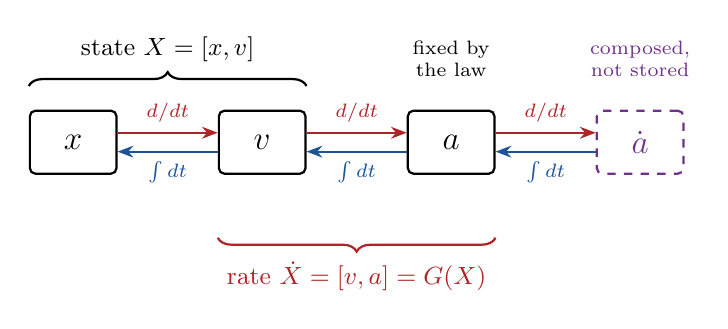
\begin{tikzpicture}[
  box/.style={draw,thick,rounded corners=2pt,minimum width=11mm,minimum height=8mm,font=\large},
  ghost/.style={draw,thick,dashed,compurple,rounded corners=2pt,minimum width=11mm,minimum height=8mm,font=\large},
  fwd/.style={-{Stealth[length=2mm]},thick,ratered},
  bwd/.style={-{Stealth[length=2mm]},thick,accblue}]
\node[box] (x) at (0,0) {$x$};
\node[box] (v) at (2.4,0) {$v$};
\node[box] (a) at (4.8,0) {$a$};
\node[ghost] (j) at (7.2,0) {$\dot a$};
\foreach \p/\q in {x/v,v/a,a/j}{
  \draw[fwd] ([yshift=1.2mm]\p.east) -- node[above,font=\scriptsize]{$d/dt$} ([yshift=1.2mm]\q.west);
  \draw[bwd] ([yshift=-1.2mm]\q.west) -- node[below,font=\scriptsize]{$\int dt$} ([yshift=-1.2mm]\p.east);}
\draw[decorate,decoration={brace,amplitude=5pt},thick] ([yshift=3mm]x.north west) -- node[above=5pt,font=\small]{state $X=[x,v]$} ([yshift=3mm]v.north east);
\draw[decorate,decoration={brace,amplitude=5pt,mirror},thick,ratered] ([yshift=-8mm]v.south west) -- node[below=5pt,font=\small,ratered]{rate $\dot X=[v,a]=G(X)$} ([yshift=-8mm]a.south east);
\node[above=3mm of a,font=\scriptsize,align=center] {fixed by\\ the law};
\node[above=3mm of j,font=\scriptsize,compurple,align=center] {composed,\\ not stored};
\end{tikzpicture}
\end{center}

\noindent The window shifts. Differentiating the state moves the same two-slot container up one rung: in $\dot X=[v,a]$, velocity occupies the position slot and acceleration the velocity slot. The link $v=\dot x$ between slots is what lets the window shift cleanly, and the law $G$ fills the upper slot from the lower pair. Integration runs the shift in reverse and needs the initial data to restore the lower slot, which is the content of Eq.~\eqref{e:4} below.

\smallskip
\noindent Acceleration is therefore the rate of the state, and the jerk $\dot a=\partial_xg\,v+\partial_vg\,a$ is already a function of $[x,v]$. Higher derivatives add no new state. The exception is degenerate: a law of third order cannot close on $[x,v]$ and forces $a$ to be promoted to independent state, and that is where the description breaks down. The Abraham--Lorentz equation of radiation reaction has runaway solutions and preacceleration~\cite{jackson}, and nondegenerate higher-derivative Lagrangians carry the Ostrogradsky instability~\cite{woodard}. The Abraham--Lorentz equation is the exception that proves the rule. It is the one equation of motion in the established canon carrying a third time derivative, and it arises by collapsing a delayed self-interaction: an extended charge responds to its own field with a finite delay, and the point limit with a local Taylor expansion of that delay produces $\dot a$~\cite{jackson}. Keeping the delay keeps the law causal with no added derivative. Fluid dynamics carries the same structure. A sphere accelerating through a viscous fluid feels the Basset--Boussinesq--Oseen history force, which weights its past acceleration by $(t-\tau)^{-1/2}$~\cite{maxey}, a fractional integral of order $\tfrac12$ of the form of Eq.~\eqref{e:20}. Gravitation has a counterpart in Mashhoon's nonlocal gravity, where history dependence enters through a constitutive relation with a causal kernel~\cite{mashhoonsym,mashhoon}. In each case memory enters as a causal-past kernel, not as another derivative slot. Accumulation proceeds in the opposite direction by integration: acceleration integrates to changes in velocity, and velocity integrates to changes in position, given the initial data. In particular,
\begin{equation}
X(t)-X(t_0)=\int_{t_0}^{t}\dot X(\tau)\,d\tau.\label{e:4}
\end{equation}
The fundamental theorem of calculus (FTC) therefore distinguishes the local differential description from its accumulated net change. Introducing a higher local derivative is not, by itself, the operation that accumulates the effects of an existing rate; as the third-order case shows, it can instead destabilize the law. Nor does the endpoint difference in \eqref{e:4} specify how intermediate events contribute to later evolution. For that, the evolving law must carry an explicit dependence on history.

A representative history functional is
\begin{equation}
M(t)=\int_{t_0}^{t}K(t,\tau)\,F\bigl(X(\tau)\bigr)\,d\tau.\label{e:5}
\end{equation}
Here $K$ is a memory kernel and $F$ specifies what aspect of the past state enters the accumulation. The distinction is precise: Eq.~\eqref{e:4} recovers net change; Eq.~\eqref{e:5} can discriminate trajectories with identical endpoints but different histories. Instantaneous dependence is a special forgetful case, represented schematically by concentration of $K(t,\tau)$ at $\tau=t$; it is not a claim that all Markov descriptions literally use delta distributions. Only two kernels make the present state sufficient. In the \emph{Dirac limit} the kernel concentrates at $\tau=t$ and nothing of the past enters: the law is forgetful. In the \emph{light-cone limit} the kernel retains every contribution of the causal past without loss, so the present state encodes the whole history: the law is faithful. Faithful here means lossless encoding in the present, not record-keeping: the past is carried by the present state itself, through the law's own accumulation, as the present pair $(\sJ,\partial_t\sJ)$ of the carrier of Sec.~3 under the second-order law at $\afrac=2$ carries a memory that reaches the whole past cone, and no separate record of each past contribution is kept. This is the usage of the companion Feynman paper. These are the only Markov limits; every kernel between them is history dependent and admits no Markov closure on the variables actually tracked. A Markovian whole generically induces such kernels in its reduced representations. For two coupled oscillators, the pair $(x_1,p_1,x_2,p_2)$ evolves Markovianly, yet eliminating the second oscillator leaves $x_1$ obeying an integro-differential equation with a memory kernel; the projection-operator formalism of Mori and Zwanzig makes this general~\cite{mori,zwanzig}. Lossy memory, between the two limits, is therefore the general form of a law on the variables actually tracked, and the Markov limits are its boundary cases. Section~2 proposes which limit a closed system can reach, and under what postulate.

\begin{symtab}{Sec.~1}
X(t) & State $[x(t),v(t)]$ & point of $M=TQ$ & \eqref{e:3}\\
x,\ v,\ a & Position, velocity $\dot x$, acceleration $\dot v$ & components of $X$, $\dot X$ & \eqref{e:3}\\
G & Law; vector field filling the rate slot & section $M\to TM$ & \eqref{e:3}\\
g(x,v) & Acceleration field, $a=g(x,v)$ & function on $M$ & \eqref{e:3}\\
X^{(n)} & $n$th time derivative of the state & recursion of $G$ & Sec.~1\\
\dot a & Jerk; fixed by $[x,v]$, not stored & derived quantity & Sec.~1\\
\tau & Integration variable (time) & real & \eqref{e:4}\\
K(t,\tau) & Memory kernel of the history functional & real kernel & \eqref{e:5}\\
F & Aspect of the past state entering $M(t)$ & map on states & \eqref{e:5}\\
M(t) & History functional & functional of the path & \eqref{e:5}\\
Q & Configuration space (distinct from $Q(x)$ of Sec.~3) & smooth manifold & \eqref{e:3}\\
\partial_x,\ \partial_v,\ \partial_\mu & Partial derivatives & differential operators & Sec.~1\\
x_1,p_1,x_2,p_2 & Positions and momenta of two coupled oscillators & real & Sec.~1\\
\end{symtab}

\section{Causal paths, composition, and transport}

Let $\mathcal S$ be a space of physical states. A \emph{causal path category} $\Path(\mathcal S)$ has admissible time-labelled states as objects, admissible histories $\gamma:X_{t_0}\to X_{t_1}$ as morphisms, identity histories as identities, and chronological concatenation as composition, in the sense in which processes form the morphisms of a category in physics, topology, logic, and computation alike~\cite{baezstay}. Thus
\begin{equation}
X_{t_0}\xrightarrow{\ \gamma_1\ }X_{t_1}\xrightarrow{\ \gamma_2\ }X_{t_2},\qquad \gamma_2\circ\gamma_1:X_{t_0}\longrightarrow X_{t_2}.\label{e:6}
\end{equation}
The FTC accumulation over such a concatenation respects interval decomposition,
\begin{equation}
\int_{t_0}^{t_2}\dot X\,dt=\int_{t_0}^{t_1}\dot X\,dt+\int_{t_1}^{t_2}\dot X\,dt.\label{e:7}
\end{equation}
The category retains the morphism, that is, the history, rather than identifying it with its endpoint difference. Composition is associative where histories are composable; this does not assert that all physical interventions commute.

For geometric accumulation, let $E\to\mathcal M$ be a bundle over spacetime, with fibers $E_x$. A contribution at $x'$ is in $E_{x'}$ and cannot generally be added directly to one at $x$. A connection supplies path-dependent parallel transport $P_\gamma:E_{x'}\to E_x$ satisfying
\begin{equation}
P_{\gamma_2\circ\gamma_1}=P_{\gamma_2}\circ P_{\gamma_1},\qquad P_{\mathrm{id}_x}=\mathrm{id}_{E_x}.\label{e:8}
\end{equation}
Thus transport is a functorial assignment on the selected path category, as a connection is a functor from paths to its structure group in gauge theory and its higher generalizations~\cite{baezhuerta}. Distinct paths can yield different transports in curved geometry. Weighting and integration are additional analytic operations; they are not implied by functoriality alone.

\smallskip
\noindent\textbf{Three levels: histories, rates, and comparison of rates.} The container picture of Sec.~1 and the transport of Eq.~\eqref{e:8} are two faces of one categorical structure, a tangent category~\cite{rosicky,cockett2014}. It has three levels.
\begin{enumerate}\itemsep2pt
\item \emph{The category: histories.} $\Path(\mathcal S)$ of Eq.~\eqref{e:6}, with states as objects and histories as morphisms. There are ordered changes but no rates.
\item \emph{The tangent category: rates.} A tangent functor $T$ with projection $p:T\Rightarrow1$ assigns to each state space $M$ its bundle of rates $TM$; for mechanics $M=TQ$ is the space of pairs $[x,v]$. A law is a section $G:M\to TM$, $p\circ G=\mathrm{id}$. This is a coalgebra for $T$: each state determines its own rate, which is what makes the law Markovian. Unfolding it,
\begin{equation*}
M\xrightarrow{\ G\ }TM\xrightarrow{\ TG\ }T^2M\xrightarrow{\ T^2G\ }T^3M\longrightarrow\cdots,
\end{equation*}
generates every higher derivative, the recursion of Sec.~1. In stream form the derivative is the shift and Taylor expansion is the map into the final coalgebra of streams~\cite{pavlovic,rutten}; Rutten's fundamental theorem $\sigma=\sigma(0)+\int\sigma'$ is the FTC with the head supplied.
\item \emph{The tangent of the tangent: laws and transport.} $T^2Q=T(TQ)$ carries two projections to $TQ$, $p_{TQ}$ and $T(p_Q)$, exchanged by the canonical flip $c:T^2\Rightarrow T^2$,
\begin{equation*}
\begin{tikzcd}[column sep=huge]
T^2Q \arrow[loop left,"c"] \arrow[r,shift left=1ex,"p_{TQ}"] \arrow[r,shift right=1ex,"T(p_Q)"'] & TQ
\end{tikzcd}
\qquad p_{TQ}\circ c=T(p_Q),\quad T(p_Q)\circ c=p_{TQ},\quad c\circ c=\mathrm{id}.
\end{equation*}
The flip is the precise form of the shifted window: it moves velocity into the position slot. A second-order law is a section $G:TQ\to T^2Q$ on which both projections agree, $p_{TQ}\circ G=T(p_Q)\circ G=\mathrm{id}$; the second equality is $v=\dot x$. The same level carries comparison of rates at different points. A connection is a connector $K:T^2M\to TM$ splitting $T^2M$ into vertical and horizontal parts through the vertical lift $\ell:T\Rightarrow T^2$, and its torsion is measured by the flip, $K-K\circ c$~\cite{cockett2017}. The parallel transport $P_\gamma$ of Eq.~\eqref{e:8} is generated at this level.
\end{enumerate}
A second-order law closes at the third level: $T^3$ adds directions that the flips only permute, and the law already determines them. A third-order law is not a coalgebra on $TQ$ at all; its carrier must be enlarged to second-order jets, which is the breakdown of Sec.~1. A history kernel is different again. It does not factor through any finite jet carrier, so its natural carrier is $\Path(\mathcal S)$ itself. Ordinary laws are coalgebras on finite jet bundles; causal accumulation is a law whose carrier is the path category. Markov processes and reaction networks already compose categorically as open systems, with black-boxing as a functor~\cite{baezfongpollard,fongspivak,baezpollardrn,hornjackson}; causal accumulation asks for the corresponding composition of non-additive functionals on $\Path(\mathcal S)$. The endpoint difference is a functor from $\Path(\mathcal S)$ to an additive group, with Eq.~\eqref{e:7} as its functoriality, while the history functional of Eq.~\eqref{e:5} is not.

\smallskip
\noindent\textbf{Three tiers of path dependence.} The contrast between Eqs.~\eqref{e:4} and \eqref{e:5} has a standard cohomological form~\cite{botttu}. Let $N$ be a smooth manifold (the state space, or spacetime $\mathcal M$), $\Omega^k(N)$ its smooth $k$-forms, and $d$ the exterior derivative, $d^2=0$. The de Rham cohomology
\begin{equation}
H^k_{\mathrm{dR}}(N)=\frac{\ker\bigl(d:\Omega^k(N)\to\Omega^{k+1}(N)\bigr)}{\operatorname{im}\bigl(d:\Omega^{k-1}(N)\to\Omega^k(N)\bigr)}\;\cong\;H^k(N;\underline{\mathbb R})\tag{8a}\label{e:8a}
\end{equation}
is isomorphic to the sheaf cohomology of the constant sheaf $\underline{\mathbb R}$: by the Poincar\'e lemma, $0\to\underline{\mathbb R}\to\Omega^0\xrightarrow{d}\Omega^1\xrightarrow{d}\cdots$ is a fine resolution, and this is de Rham's theorem in sheaf form~\cite{botttu}. A 1-form $\omega$ integrated along a history $\gamma$ falls into one of three tiers.
\begin{enumerate}\itemsep1pt
\item \emph{Exact}, $\omega=df$. Then
\begin{equation}
\int_\gamma df=f\bigl(\gamma(1)\bigr)-f\bigl(\gamma(0)\bigr),\tag{8b}\label{e:8b}
\end{equation}
which sees only the endpoints. Eq.~\eqref{e:4} is this tier, componentwise in the state coordinates, and Eq.~\eqref{e:7} is its additivity.
\item \emph{Closed}, $d\omega=0$. For histories $\gamma,\gamma'$ with common endpoints,
\begin{equation}
\int_\gamma\omega-\int_{\gamma'}\omega=\oint_{\gamma'^{-1}\circ\gamma}\omega,\tag{8c}\label{e:8c}
\end{equation}
which vanishes when the loop is contractible and in general depends only on $[\omega]\in H^1_{\mathrm{dR}}(N)$ paired with the homology class of the loop. On every contractible patch $\omega$ has a primitive; the local primitives agree on overlaps up to constants, and $[\omega]$ is exactly the obstruction to gluing them into one global $f$. This is local-to-global failure in the sense of sheaf cohomology: path dependence invisible on any patch and carried entirely by topology.
\item \emph{Not closed}, $d\omega\ne0$. For a loop bounding a surface $\Sigma$,
\begin{equation}
\oint_{\partial\Sigma}\omega=\int_\Sigma d\omega,\tag{8d}\label{e:8d}
\end{equation}
so path dependence appears already on arbitrarily small loops and is measured pointwise by $d\omega$.
\end{enumerate}
For generic kernel $K$ and aspect $F$, the history functional of Eq.~\eqref{e:5} lies outside all three tiers. It is not $\int_\gamma\omega$ for any 1-form $\omega$ on the state space: it depends on the time labelling of $\gamma$ and not only on its image, and through $K(t,\tau)$ on the evaluation time $t$ as well as on the path. The decisive difference is additivity. In all three tiers the line integral is additive under concatenation, $\int_{\gamma_2\circ\gamma_1}\omega=\int_{\gamma_1}\omega+\int_{\gamma_2}\omega$, so each defines a functor from $\Path(N)$ to the additive group $\mathbb R$; Eq.~\eqref{e:7} is this additivity. Because $K(t,\tau)$ depends on the evaluation time $t$, the contribution of an earlier segment changes when the history is extended, so $M$ is not additive under concatenation and is not a functor to any additive group. This is the precise sense in which its carrier is $\Path(\mathcal S)$ rather than a cohomology theory of $\mathcal S$.

\smallskip
\noindent\textbf{Neither faithful nor forgetful.} A functor is faithful when it keeps distinct morphisms distinct. The endpoint difference is not faithful: histories with common endpoints have the same image. Neither is the physical readout of Sec.~3 forgetful in the sense of discarding all history. The left closure $\sJ\sJ^\dagger$ retains the order of left-acting transports (Eq.~\eqref{e:47}), while it is invariant under right unitaries and cancels central phases (Eq.~\eqref{e:54}); it therefore distinguishes some histories and identifies others. Four steps place this between the two Markov limits of Sec.~1.

\Derived \textit{Lossless transport, and no cross product on the carrier.} For $\dot x=\Omega x$,
\begin{equation*}
\frac{d}{dt}|x|^2=x^{\mathsf T}\bigl(\Omega+\Omega^{\mathsf T}\bigr)x ,
\end{equation*}
which vanishes for every $x$ exactly when $\Omega$ is antisymmetric, in any dimension. In three dimensions every such generator is a cross product, $\Omega x=\vec\theta\times x$. A cross product, a nonzero bilinear product orthogonal to both factors with $|u\times v|^2=|u|^2|v|^2-(u\cdot v)^2$, exists only in dimensions three and seven~\cite{browngray}. The carrier $\mathbb C\otimes\mathbb H$ has complex dimension four and real dimension eight, so it carries no cross product. Among its actions on itself by left multiplication, $\sJ\mapsto G\sJ$, the lossless ones are the unitary $G$, generated by the anti-Hermitian slice $\mathfrak u(2)$; they preserve both the trace and the determinant of the closure (Eq.~\eqref{e:52}). A general norm-preserving map of the eight real components, generated by $\mathfrak{so}(8)$, preserves the trace but not in general the determinant. Traceless Hermitian generators, the boosts, preserve the determinant and change the trace by the state-dependent amount $\delta x^0=\varepsilon\,\vec\beta\cdot\vec x$ (Eq.~\eqref{e:52}); the remaining Hermitian direction $I_2$ is a dilation and rescales both. The antisymmetric part of the product is the commutator $[\sJ,K]=\sJ K-K\sJ$, defined on the whole carrier but a cross product only on the three vector directions $e_j$, where $\tfrac12[e_j,e_k]=\varepsilon_{jk\ell}e_\ell$ (Eq.~\eqref{e:11}); the term $i\,\vec b\times\vec b^{\,*}$ of Eq.~\eqref{e:44} is this restriction. The scalar trace $\tfrac12\tr\varrho$ discards it, while an effect $E_m$ that is not a multiple of $I_2$ reads it and so distinguishes $\sJ\sJ^\dagger$ from $\sJ^\dagger\sJ$ (Eq.~\eqref{e:46}).

\Derived \textit{Contraction to rank one is many-to-one.} A contraction from a rank-two object to a rank-one object is a linear map with a nontrivial kernel and cannot be inverted. The acceleration $a^\mu=\Omega^\mu{}_\nu u^\nu$ of Sec.~3.2.6 does not determine the pair $(\Omega,u)$. The closure $\varrho=\sJ\sJ^\dagger$ is quadratic rather than linear, and is many-to-one because it is constant on every right-unitary orbit $\sJ\mapsto\sJ U$ (Eq.~\eqref{e:45}): it sends the eight real components of $\sJ$ to four. The scalar trace $\tfrac12\tr\varrho=x^0$ discards the spatial components and with them the inter-channel cross terms, including the antisymmetric term $i\,\vec b\times\vec b^{\,*}$ of Eq.~\eqref{e:44}; an effect $E_m$ that is not a multiple of $I_2$ still reads them (Sec.~3.1).

\Proposed \textit{Bounded retrievable capacity and the Landauer bound.} A physical memory retains a bounded amount of retrievable history: a system of bounded size and energy has bounded entropy~\cite{bekenstein1981}, so its records resolve only finitely many past distinctions. Finite storage is a capacity, not an energy cost; the energy cost attaches to erasure. A record held within finite capacity must be overwritten as new contributions arrive, and each bit irreversibly erased dissipates at least $k_BT\ln2$ into the complement~\cite{landauer,bennett2003}. Since the contraction to rank one is many-to-one, a faithful, lossless encoding, whether in the present state or in a record, would also have to keep the components each contraction discards, and it is erasing those records, not evaluating the contraction, that carries the cost. This loss is operational: contributions of the causal past are retained ever more weakly, as under a power-law kernel, and fall below the resolution of any finite record without any two global states being merged exactly.

\Proposed \textit{Lossy memory.} Open systems with an energy budget carry lossy memory between the two limits, retaining part of the past at a cost and letting the rest decay. This is the regime of the examples already given: the radiating charge, whose delayed self-interaction carries energy away (Sec.~1); the Basset--Boussinesq--Oseen force, whose power-law weighting of past acceleration is paid for by viscous dissipation (Sec.~1); and human memory, which follows power laws on a budget of roughly 20 watts (Introduction, Sketch~4). The structures of this note are thus neither faithful to every history nor forgetful of all of them.

\smallskip
\noindent\textbf{Closed systems.} Operational loss in a subsystem does not by itself exclude the light-cone limit for the whole: under unitary or Hamiltonian evolution the global map is a bijection, and what a subsystem erases is moved into its complement rather than destroyed.

\Proposed \textit{Postulate: global non-injectivity.} Fundamental causal evolution is not injective: distinct histories of the whole can arrive at the same global state. This departs from global unitarity and from Liouville's theorem, and the present note does not supply its mechanism. It is constrained by conservation: any evolution law for the density matrix more general than the Schr\"odinger equation violates either locality or energy--momentum conservation~\cite{bankssusskindpeskin}, so a realization of the postulate must state how it meets that argument.

\Derived \textit{The finite deterministic case.} Let $\mathcal S$ be finite, and let deterministic maps $\Psi_t:\mathcal S\to\mathcal S$ compose to $\Psi_{t:0}=\Psi_t\circ\cdots\circ\Psi_1$. The image $\Psi_{t:0}(\mathcal S)$, the set of global states still reachable at step $t$, cannot grow in cardinality, so at most $|\mathcal S|-1$ steps can strictly reduce it, and at most $\log_2|\mathcal S|$ bits of initial distinguishability can be lost in all; the two are different counts. Two states once sent to the same image stay merged under every later $\Psi_{m:0}$. For an autonomous law, $\Psi_t=\Psi$, every trajectory enters the recurrent set $\mathcal R$, on which $\Psi$ is a bijection, within $|\mathcal S|-|\mathcal R|$ steps. That the present determines earlier states within $\mathcal R$ is a property of the law, injectivity, not an operation anyone can perform on the universe; it is not the faithful accumulation of Sec.~1, in which the present state encodes every contribution of the causal past without loss through the law's own accumulation; injectivity on $\mathcal R$ encodes earlier states only from entry into $\mathcal R$ on, and it restores none of the distinctions merged before entry. The bound limits repeated exact global merging; it does not limit the operational loss above, which continues within any finite capacity.

\Proposed \textit{Which Markov limit a closed system reaches.} Under the postulate some distinct histories of the whole merge, and merged histories stay merged, so from the first merger on the present state no longer carries the whole history: the closed system cannot be in the light-cone limit, and of the two Markov limits only the Dirac limit remains. Without the postulate the global map is a bijection: earlier global states are determined by the present in principle, though no observer inside the universe can run it backward, and by the previous paragraph this is not by itself faithful accumulation.

\smallskip
\noindent\textbf{Flat transport and local systems.} The same tiers apply to the transport of Eq.~\eqref{e:8}. If the connection is flat, $P_\gamma$ depends only on the homotopy class of $\gamma$ with fixed endpoints, so transport factors through the fundamental groupoid $\Pi_1(\mathcal M)$; equivalently, the sheaf of locally parallel sections of $E$ is locally constant, a local system~\cite{botttu}. Holonomy around a noncontractible loop is then topological, the second tier. Curvature is the third tier: it fixes the holonomy around loops that bound, to leading order in the area they enclose.

\smallskip
\noindent\textbf{Divergence.} N.~Ghani asked whether the local-to-global failure measured by sheaves is related to the divergence operator on vector fields~\cite{ghani}. It is, one degree up the same complex. On an oriented Riemannian 3-manifold,
\begin{equation}
\operatorname{div}v=\star\,d\star v^\flat,\tag{8e}\label{e:8e}
\end{equation}
so $v$ is divergence-free exactly when its flux 2-form $\star v^\flat$ is closed. It is then locally a curl, by the Poincar\'e lemma, and the class $[\star v^\flat]\in H^2_{\mathrm{dR}}$ is the obstruction to a global vector potential. Gauss's law is the standard instance; Sec.~7 sketches it and its role for conservation in CAL.



\begin{symtab}{Sec.~2}
\mathcal S & Space of physical states & set or space & Sec.~2\\
\Path(\mathcal S) & Causal path category & category & \eqref{e:6}\\
\gamma & Admissible history & morphism of $\Path(\mathcal S)$ & \eqref{e:6}\\
E\to\mathcal M & Bundle over spacetime, fibers $E_x$ & fiber bundle & \eqref{e:8}\\
P_\gamma & Parallel transport along $\gamma$ & linear map $E_{x'}\to E_x$ & \eqref{e:8}\\
T & Tangent functor & endofunctor & Sec.~2\\
p & Tangent projection & natural transformation $T\Rightarrow1$ & Sec.~2\\
c & Canonical flip on $T^2$ & natural iso $T^2\Rightarrow T^2$ & Sec.~2\\
\ell & Vertical lift & natural transformation $T\Rightarrow T^2$ & Sec.~2\\
K & Connector of a connection (distinct from Eq.~\eqref{e:5}) & map $T^2M\to TM$ & Sec.~2\\
N & Manifold: state space or spacetime & smooth manifold & \eqref{e:8a}\\
\Omega^k(N),\ d & $k$-forms; exterior derivative (distinct from $\Omega^\mu{}_\nu$ of Sec.~3.2.6) & vector space; $d^2=0$ & \eqref{e:8a}\\
H^k_{\mathrm{dR}}(N) & de Rham cohomology & real vector space & \eqref{e:8a}\\
\underline{\mathbb R} & Constant sheaf & sheaf on $N$ & \eqref{e:8a}\\
\omega,\ f & 1-form; function (primitive) & $\Omega^1(N)$; $\Omega^0(N)$ & \eqref{e:8b}\\
\Sigma & Surface bounded by a loop & 2-chain & \eqref{e:8d}\\
\Pi_1(\mathcal M) & Fundamental groupoid & groupoid & Sec.~2\\
\star,\ v^\flat & Hodge star; metric dual of $v$ & operator; 1-form & \eqref{e:8e}\\
s & Age of a contribution, $t-\tau$ & positive real & Sec.~2\\
\sigma & Stream in Rutten's calculus (distinct from the Pauli $\sigma_j$) & sequence & Sec.~2\\
\Gamma & Gamma function & special function & Sec.~2\\
\partial & Boundary operator on chains & linear map, $\partial^2=0$ & \eqref{e:8d}\\
\Omega & Generator in $\dot x=\Omega x$ (distinct from $\Omega^k(N)$) & real square matrix & Sec.~2\\
k_B,\ T & Boltzmann constant; temperature ($T$ distinct from the tangent functor) & positive reals & Sec.~2\\
\Psi_t,\ \Psi_{t:0} & Deterministic global update at step $t$; its composite (distinct from the spinor $\psi$) & maps $\mathcal S\to\mathcal S$ & Sec.~2\\
|\mathcal S| & Number of global states in the finite case & positive integer & Sec.~2\\
\mathcal R & Recurrent set of an autonomous update & subset of $\mathcal S$ & Sec.~2\\
\end{symtab}

\section{The biquaternionic source carrier}

The source algebra may be specified independently of solving CAL. For each channel $a\in\{0,1,2,3\}$, set
\begin{equation}
Z_a(x)\coloneqq A_a(x)e^{-H_a(x)/\tau_E}+B_a(x)e^{iS_a(x)/\hbareff},\qquad A_a+B_a=1,\quad A_a\in[0,1],\qquad \tau_E>0.\label{e:10}
\end{equation}
The ratios in the exponentials are dimensionless: $H_a/\tau_E$ is an energy ratio, while $S_a/\hbareff$ is an action ratio. The energy scale $\tau_E$ is distinct from the proper-time argument $\tau$ of CAL. Each channel therefore holds the two standard weights of physics. The decay factor $e^{-H_a/\tau_E}$ is a Boltzmann weight, with $\tau_E$ in the role of $k_BT$, the summand of a statistical partition function $\sum e^{-H/k_BT}$. The phase factor $e^{iS_a/\hbareff}$ is the weight Feynman assigns to a history, the integrand of the path integral $\int e^{iS/\hbar}$~\cite{feynman}. The two are related by the substitution $1/k_BT\to1/(i\hbar)$, which turns $e^{-E/k_BT}$ into $e^{iS/\hbar}$ and which Baez and Pollard use to treat the path integral as a partition function, with \emph{quantropy} as the corresponding analogue of entropy~\cite{quantropy}. The same correspondence runs between stochastic and quantum mechanics more broadly, where probability evolution and amplitude evolution share generators and ladder-operator techniques~\cite{baezbiamonte,doi}. Eq.~\eqref{e:10} carries both weights in one channel amplitude, and Eq.~\eqref{e:22} below identifies the relative phase between the two sectors after accumulation as the Wick angle $\theta=\pi\afrac/2$. A single $Z_a$ is a weight, not a sum: it becomes a partition function or a path integral only when summed over states or histories, and the sum CAL performs is the causal accumulation of Eq.~\eqref{e:9} over $J^-(x)$.

\noindent\textbf{Sector weights.} The constraint $A_a+B_a=1$, $A_a\in[0,1]$, holds independently in each channel. It does not make $Z_a$ real: $Z_a$ is complex whenever $S_a/\hbareff\notin\pi\mathbb Z$. What it fixes is the following. First, $A_a\in[0,1]$ makes both sector weights real and nonnegative, so the relative argument between the two sectors is exactly $S_a/\hbareff$, the only invariant that distinguishes configurations; the condition $A_a+B_a=1$ read over $\mathbb C$ would not do this. Second, $Z_a$ is a convex combination of $e^{-H_a/\tau_E}$ and $e^{iS_a/\hbareff}$, so $Z_a=1$ at the reference point $H_a=S_a=0$ and $|Z_a|\le1$ wherever $H_a\ge0$. The constraint could be relaxed to complex $A_a,B_a$. The cost is a constant offset $\arg(B_a/A_a)$ in the relative argument, which is then no longer fixed by the action alone, together with the loss of the reference normalization.

With the quaternion matrix basis
\begin{equation}
e_0=I_2,\qquad e_j=-i\sigma_j\ \ (j=1,2,3),\qquad e_je_k=-\delta_{jk}I_2+\varepsilon_{jk\ell}e_\ell,\label{e:11}
\end{equation}
assemble the four complex amplitudes into one carrier,
\begin{equation}
\sJ(Z)\coloneqq\sum_{a=0}^{3}Z_ae_a\in\mathbb C\otimes\mathbb H\cong M_2(\mathbb C).\label{e:12}
\end{equation}
This matrix carrier is associative. The corresponding indexed source is assembled at fixed tensor slots as $\sJ^{\mu\nu}{}_{\rho\sigma}=\sum_aJ^{\mu\nu a}{}_{\rho\sigma}e_a$. Equation \eqref{e:10} does not automatically identify $Z_a$ with every indexed coefficient $J^{\mu\nu a}{}_{\rho\sigma}$; such an assignment belongs to a chosen source profile.

\subsection*{Positive closure and the Born rule}

Hermitian conjugation of the entire matrix carrier gives
\begin{equation}
\varrho=\sJ\sJ^\dagger\succeq0,\qquad \frac12\tr(\varrho)=\sum_{a=0}^{3}|Z_a|^2.\label{e:13}
\end{equation}
The second identity follows from the orthogonality of the quaternion basis under the scalar trace; it is a consequence of the geometric product, not an assumed inner product on an ambient state space. For measurement effects $E_m\succeq0$ with $\sum_mE_m=I_2$, define
\begin{equation}
w_m=\tr(E_m\varrho),\qquad p_m=\frac{\tr(E_m\sJ\sJ^\dagger)}{\tr(\sJ\sJ^\dagger)},\qquad \sum_mp_m=1,\label{e:14}
\end{equation}
provided $\sJ\neq0$. These are nonnegative normalized probabilities. For a rank-one carrier $\sJ=\psi\eta^\dagger$ with $\eta^\dagger\eta=1$ and rank-one effect $E_m=\phi_m\phi_m^\dagger$, Eq.~\eqref{e:14} specializes to
\begin{equation}
p_m=\frac{|\phi_m^\dagger\psi|^2}{\psi^\dagger\psi}.\label{e:15}
\end{equation}
This is the Born rule. The assumptions are the choice of positive effects and trace evaluation; the squared-amplitude form follows algebraically from the biquaternionic closure.

\subsection*{Lorentzian determinant and the retained four-vector}

The same $M_2(\mathbb C)$ carrier contains the real four-dimensional Hermitian slice
\begin{equation}
X=X^\dagger=x^\mu\sigma_\mu=\begin{pmatrix}x^0+x^3&x^1-ix^2\\x^1+ix^2&x^0-x^3\end{pmatrix},\qquad x^\mu\in\mathbb R.\label{e:16}
\end{equation}
Its determinant is exactly
\begin{equation}
Q(x)\coloneqq\det X=(x^0)^2-(x^1)^2-(x^2)^2-(x^3)^2,\qquad \frac12\frac{\partial^2Q}{\partial x^\mu\partial x^\nu}=\eta_{\mu\nu}=\mathrm{diag}(1,-1,-1,-1).\label{e:17}
\end{equation}
Thus Lorentzian signature comes from the determinant quadratic form on the Hermitian slice, not from positivity by itself. For $G\in SL(2,\mathbb C)$, congruence $X\mapsto GXG^\dagger$ preserves $\det X$ and induces the proper orthochronous Lorentz action (with $G$ and $-G$ equivalent)~\cite{baylis,penrose}.

The positive closure $\varrho=\sJ\sJ^\dagger$ belongs to this Hermitian slice. Its four real coefficients are retained by
\begin{equation}
\varrho=x^\mu\sigma_\mu,\qquad x^\mu=\frac12\tr(\sigma^\mu\varrho),\qquad \det\varrho=\eta_{\mu\nu}x^\mu x^\nu=|\det\sJ|^2.\label{e:18}
\end{equation}
Here $\sigma^\mu=(I_2,\sigma_1,\sigma_2,\sigma_3)$ denotes the \emph{trace-dual} basis, not index-raising by $\eta$. Metric lowering instead gives $x_\mu=\eta_{\mu\nu}x^\nu$, represented on matrices by
\begin{equation}
\adj(\varrho)=(\tr\varrho)I_2-\varrho=x_\mu\sigma^\mu,\qquad \varrho\,\adj(\varrho)=(\det\varrho)I_2.\label{e:19}
\end{equation}
Since $\varrho\succeq0$, $x^0\ge0$ and $(x^0)^2\ge\|\boldsymbol x\|^2$: its image lies in the future Lorentz cone, with nonzero rank-one closures null and positive rank-two closures timelike. The null closures $\psi\psi^\dagger$ are the spinor factorization of null vectors that twistor theory takes as primitive~\cite{penrosetwistor}. The determinant supplies the metric while trace effects supply the Born readout; they are distinct constructions on the same carrier.

\subsection*{Fractional accumulation and the closure}

Let the carrier itself be integrated to order $\afrac$, the interaction depth of Eq.~\eqref{e:9}. Linearize the exponents of Eq.~\eqref{e:10} about the present, $-H_a/\tau_E\approx c_a+\lambda_at$ and $S_a/\hbareff\approx d_a+\omega_at$, so that $\lambda_a=-\partial_tH_a/\tau_E$ is the decay rate and $\omega_a=\partial_tS_a/\hbareff$ the phase rate of channel $a$, with $\lambda_a>0$ so that earlier contributions are exponentially suppressed relative to the present, and $\omega_a\neq0$, since for a stationary phase sector the integral of Eq.~\eqref{e:20} diverges for every $\alpha>0$. Then
\begin{equation*}
Z_a(t)=\hat A_ae^{\lambda_at}+\hat B_ae^{i\omega_at},\qquad \hat A_a=A_ae^{c_a}\ge0,\qquad \hat B_a=B_ae^{id_a},\quad |\hat B_a|=B_a .
\end{equation*}
The constants are carried in the prefactors rather than absorbed into $A_a$ and $B_a$, which would break $A_a+B_a=1$; the constraint lives on $A_a,B_a$, not on $\hat A_a,\hat B_a$. The past-supported (Weyl) integral of order $\alpha\equiv\afrac$~\cite{samko,podlubny},
\begin{equation}
(I^\alpha f)(t)=\frac1{\Gamma(\alpha)}\int_{-\infty}^{t}(t-\tau)^{\alpha-1}f(\tau)\,d\tau,\qquad I^\alpha e^{st}=s^{-\alpha}e^{st}\quad(\Real s>0),\label{e:20}
\end{equation}
with $I^0$ the identity and, for the oscillatory sector, defined as the limit $s=\epsilon+i\omega_a$, $\epsilon\to0^+$ (for $\alpha\ge1$ the integral diverges at $\epsilon=0$ and the limit defines the value), acts on the two sectors as
\begin{equation}
I^\alpha Z_a=\hat A_a\lambda_a^{-\alpha}e^{\lambda_at}+\hat B_a(i\omega_a)^{-\alpha}e^{i\omega_at},\qquad (i\omega_a)^{-\alpha}=|\omega_a|^{-\alpha}e^{-i\pi\alpha\,\mathrm{sgn}(\omega_a)/2}.\label{e:21}
\end{equation}
The decay sector is rescaled by a positive real factor at every order. The phase sector is rescaled and rotated by $e^{-i\pi\alpha\,\mathrm{sgn}(\omega_a)/2}$: a quarter turn at $\alpha=1$, and at $\alpha=2$ a half turn, $(i\omega_a)^{-2}=-\omega_a^{-2}$. The two sectors sit at $s=\lambda_a$ and $s=i\omega_a$, separated in the frequency plane by the quarter turn of Wick rotation. The map $s\mapsto s^{-\alpha}$ carries that quarter turn into the relative phase between the accumulated sectors,
\begin{equation}
\theta=\frac{\pi\alpha}{2},\qquad \alpha\equiv\afrac,\label{e:22}
\end{equation}
so $\theta$ is the Wick angle after accumulation of order $\alpha$: at $\alpha=1$ it is the Wick rotation itself, $\theta=\pi/2$; at $\alpha=2$ it is $\theta=\pi$, the order-two sign; for $0<\alpha<1$ it runs from relaxation toward the first-order Schr\"odinger corner, reached as $\alpha\to1^-$, where the history weight $1-\afrac$ of Eq.~\eqref{e:9} vanishes and the present decouples from the past; and for $1<\alpha<2$ it runs from that first-order corner to the second-order wave regime at $\alpha=2$. Because the basis $e_a$ is constant, the accumulation acts channel by channel on the carrier,
\begin{equation}
\sJ^{(\alpha)}\coloneqq\sum_{a=0}^{3}(I^\alpha Z_a)\,e_a=I^\alpha\sJ,\qquad \varrho^{(\alpha)}\coloneqq\sJ^{(\alpha)}\sJ^{(\alpha)\dagger}\succeq0.\label{e:23}
\end{equation}
By Eq.~\eqref{e:13},
\begin{equation}
\tfrac12\tr\varrho^{(\alpha)}=\sum_{a=0}^{3}\bigl|I^\alpha Z_a\bigr|^2,\label{e:24}
\end{equation}
with, for each channel,
\begin{equation}
\bigl|I^\alpha Z_a\bigr|^2=\hat A_a^2\lambda_a^{-2\alpha}e^{2\lambda_at}+B_a^2|\omega_a|^{-2\alpha}+2\Real\Bigl[\hat A_a\hat B_a^*\lambda_a^{-\alpha}|\omega_a|^{-\alpha}e^{i\pi\alpha\,\mathrm{sgn}(\omega_a)/2}e^{(\lambda_a-i\omega_a)t}\Bigr].\label{e:25}
\end{equation}
The closure $\sJ\sJ^\dagger$ is therefore where the integration effect is resolved. First, the trace annihilates every inter-channel cross term $Z_aZ_b^*e_ae_b^\dagger$, $a\ne b$, identically and for every order, by the orthogonality used in Eq.~\eqref{e:13}. Second, in the sector-pure terms the integration phase meets its own conjugate, $(i\omega_a)^{-\alpha}\bigl[(i\omega_a)^{-\alpha}\bigr]^*=|\omega_a|^{-2\alpha}$, so the rotation, including the order-two sign, cancels and these terms are positive at every order. In the trace, the rotation survives only as the relative phase $e^{i\theta\,\mathrm{sgn}(\omega_a)}$, with $\theta$ the accumulated Wick angle of Eq.~\eqref{e:22}, of the intra-channel decay--phase interference term; at $\alpha=2$ that term reverses sign relative to $\alpha=0$. The inter-channel products, with their rotation phases, do remain in the spatial components $x^j=\frac12\tr(\sigma^j\varrho^{(\alpha)})$; it is the scalar trace, the normalization in Eq.~\eqref{e:14}, that removes them. Since $\varrho^{(\alpha)}$ is again a positive closure, Eqs.~\eqref{e:13}--\eqref{e:19} hold with $\sJ\to\sJ^{(\alpha)}$: the Born-normalized form $\varrho^{(\alpha)}/\tr\varrho^{(\alpha)}$ is again a valid state (the trace itself is rescaled by the accumulation), and the determinant identity $\det\varrho^{(\alpha)}=|\det\sJ^{(\alpha)}|^2$ and the future-cone property hold under fractional accumulation of any order. The linearization is local; for general $H_a(x)$ and $S_a(x)$ the rotation becomes path-dependent, which is the role of the transport factors in Eq.~\eqref{e:9}. The Weyl integral, by contrast, runs over the whole past, so Eq.~\eqref{e:21} is exact only when the exponents are linear over the entire support of the kernel. For $\alpha>1$ the weight $(t-\tau)^{\alpha-1}$ grows with age, so the far past, where the linearization is least accurate, carries the most weight.

\noindent\textbf{Covariant form over the past cone.} Eq.~\eqref{e:20} integrates along time. A plain integration of a spatially uniform source over the past cone $J^-(x)$, the domain of Eq.~\eqref{e:9}, weights a contribution of age $\Delta t=t-t'$ by the volume $\frac{4\pi}{3}(\Delta t)^3$ of the past ball, and so turns the phase sector by $2\pi$ rather than $\pi/2$. The covariant form of Eq.~\eqref{e:20}, the integration of order $\alpha$ over the cone, is instead the Lorentzian Riesz potential~\cite{riesz},
\begin{equation*}
(R^\alpha f)(x)=\frac{1}{H_4(\alpha)}\int_{J^-(x)}\tau(x,x')^{\alpha-4}f(x')\,d^4x',\qquad H_4(\alpha)=\pi\,2^{\alpha-1}\,\Gamma\bigl(\tfrac{\alpha}{2}\bigr)\,\Gamma\bigl(\tfrac{\alpha-2}{2}\bigr),
\end{equation*}
with $\tau(x,x')$ the proper time between $x'$ and $x$. On a spatially uniform source it reduces exactly to Eq.~\eqref{e:20}. Integrations compose by adding their orders, $R^\alpha R^\beta=R^{\alpha+\beta}$, so two integrations of order one are one integration of order two. A timelike mode $e^{i(\omega t-\vec p\cdot\vec x)}$, $|\vec p|<|\omega|$, is multiplied by $\bigl(\omega^2-|\vec p|^2\bigr)^{-\alpha/2}e^{-i\pi\alpha\,\mathrm{sgn}(\omega)/2}$: the rotation of Eq.~\eqref{e:21}, with a boost-invariant modulus. The decay sector stays real and positive, and a spacelike mode is not rotated. For $\alpha\le2$, which includes the range $0\le\afrac\le2$, the kernel $\tau^{\alpha-4}$ is not integrable at the light cone, and $R^\alpha$ is defined by analytic continuation in $\alpha$; at $\alpha=2$ its kernel is $\delta(\Delta t-|\vec x-\vec x'|)/(4\pi|\vec x-\vec x'|)$, supported on the light cone itself. Since $R^2$ is the delayed inverse of $\Box$, the order of integration is capped at $2$ for the same reason laws close at second order: $R^\alpha$ with $\alpha>2$ inverts $\Box^{\alpha/2}$, a higher-derivative operator of the kind excluded in Sec.~1. This is the covariant form of the integration of the carrier, not the history kernel $k$ of Eq.~\eqref{e:9}: $k$ is a separate object, chosen independently of $\afrac$, and taking $k=\tau^{\afrac-4}/H_4(\afrac)$ together with the affine weights $\afrac$ and $\afrac-1$ would count the order twice.

\begin{symtab}{Sec.~3}
Z_a & Channel amplitude & complex scalar field & \eqref{e:10}\\
A_a,\ B_a & Decay and phase sector weights, $A_a+B_a=1$ & reals in $[0,1]$ & \eqref{e:10}\\
\hat A_a,\ \hat B_a & Linearized prefactors $A_ae^{c_a}$, $B_ae^{id_a}$ & nonnegative real; complex & \eqref{e:21}\\
c_a,\ d_a & Constant parts of the linearized exponents & real & \eqref{e:21}\\
H_a,\ S_a & Energy and action functions & real & \eqref{e:10}\\
\tau_E,\ \hbareff & Energy scale; effective action scale & positive reals & \eqref{e:10}\\
e_0,\ e_j & Quaternion basis $I_2$, $-i\sigma_j$ & $2\times2$ matrices & \eqref{e:11}\\
\sigma_j & Pauli matrices & Hermitian $2\times2$ & \eqref{e:11}\\
\varepsilon_{jk\ell} & Levi-Civita symbol & totally antisymmetric & \eqref{e:11}\\
\mathbb H & Quaternion algebra & real associative algebra & \eqref{e:12}\\
\sJ & Carrier $\sum_aZ_ae_a$ & element of $M_2(\mathbb C)$ & \eqref{e:12}\\
\varrho & Positive closure $\sJ\sJ^\dagger$ ($\rho$ is an index) & positive semidefinite Hermitian & \eqref{e:13}\\
E_m & Measurement effect & positive Hermitian, $\sum_mE_m=I_2$ & \eqref{e:14}\\
w_m,\ p_m & Effect weight; Born probability & real; real in $[0,1]$ & \eqref{e:14}\\
\psi,\ \eta,\ \phi_m & Spinor, reference leg, effect vector & vectors in $\mathbb C^2$ & \eqref{e:15}\\
X=x^\mu\sigma_\mu & Hermitian slice element & real four-vector as matrix & \eqref{e:16}\\
Q(x) & Determinant quadratic form $\det X$ (distinct from configuration space $Q$) & quadratic form & \eqref{e:17}\\
\eta_{\mu\nu} & Minkowski metric & symmetric bilinear form & \eqref{e:17}\\
G & Element acting by congruence $X\mapsto GXG^\dagger$ (distinct from the law) & $SL(2,\mathbb C)$ element & Sec.~3\\
SL(2,\mathbb C) & Determinant-one complex matrices & Lie group & Sec.~3\\
x^\mu & Closure vector, $\frac12\tr(\sigma^\mu\varrho)$ & future-causal vector & \eqref{e:18}\\
\sigma^\mu & Trace-dual basis $(I_2,\vec\sigma)$ & Hermitian $2\times2$ & \eqref{e:18}\\
x_\mu & Metric dual of $x^\mu$ & covector & \eqref{e:19}\\
\adj & Adjugate $(\tr X)I_2-X$ & linear map on $M_2(\mathbb C)$ & \eqref{e:19}\\
I^\alpha & Weyl fractional integral of order $\alpha\equiv\afrac$ & linear operator & \eqref{e:20}\\
R^\alpha,\ H_4(\alpha) & Lorentzian Riesz potential of order $\alpha$ over $J^-(x)$; its normalization (distinct from $H_a$) & linear operator; real & Sec.~3\\
\Delta t & Age $t-t'$ of a contribution & positive real & Sec.~3\\
\vec p & Spatial wavevector of a mode & real three-vector & Sec.~3\\
\lambda_a,\ \omega_a & Decay rate; frequency & real & \eqref{e:21}\\
\theta & Accumulated Wick angle $\pi\alpha/2$ & angle & \eqref{e:22}\\
\sJ^{(\alpha)},\ \varrho^{(\alpha)} & Accumulated carrier and closure & as $\sJ$, $\varrho$ & \eqref{e:23}\\
J^{\mu\nu a}{}_{\rho\sigma} & Indexed source current & indexed tensor field & \eqref{e:9}\\
\afrac & Interaction depth; fractional order of accumulation relative to the evaluating state & real scalar & \eqref{e:9}\\
\tau & Proper time between $x'$ and $x$ (distinct from Eq.~\eqref{e:4}) & real & \eqref{e:9}\\
J^-(x) & Causal past of $x$ & subset of spacetime & \eqref{e:9}\\
\mu,\nu,\alpha,\rho,\ldots & Spacetime indices & index $0,\dots,3$ & \eqref{e:9}\\
a,b,c & Internal channel indices & index $0,\dots,3$ & \eqref{e:9}\\
\delta_{jk} & Kronecker delta & symbol & \eqref{e:11}\\
\hbar & Planck's constant & positive real & Sec.~3\\
s & Complex frequency in $I^\alpha e^{st}=s^{-\alpha}e^{st}$ (distinct from age $s$ of Sec.~2) & complex & \eqref{e:20}\\
\epsilon & Regulator, $s=\epsilon+i\omega_a$ with $\epsilon\to0^+$ & positive real & \eqref{e:20}\\
\end{symtab}

\subsection{Scalar--traceless splitting: why the two readouts share a cone}

The carrier in \eqref{e:11}--\eqref{e:12} already distinguishes one scalar channel direction from three traceless directions. In the anti-Hermitian Lie-algebra convention,
\begin{equation}
\mathfrak u(2)=\mathfrak u(1)\oplus\mathfrak{su}(2),\qquad \mathfrak u(1)=\mathbb R(iI_2),\qquad \mathfrak{su}(2)=\spanop_{\mathbb R}\{-i\sigma_1,-i\sigma_2,-i\sigma_3\}.\label{e:26}
\end{equation}
Thus $e_0=I_2$ spans the scalar direction (identified with $\mathfrak u(1)$ after multiplication by $i$), while $e_j=-i\sigma_j$ span $\mathfrak{su}(2)$. These are real directions; complex amplitudes $Z_a$ extend the basis to $\mathbb C\otimes\mathbb H\simeq M_2(\mathbb C)$. A general $J$ is not itself an element of $\mathfrak u(2)$.

The positive closure belongs instead to the Hermitian slice $i\mathfrak u(2)$. Its expansion, trace and determinant are
\begin{align}
\varrho&=JJ^\dagger=x^0I_2+\vec x\cdot\vec\sigma,\qquad x^0=\tfrac12\tr\varrho,\qquad x^j=\tfrac12\tr(\sigma_j\varrho),\label{e:27}\\
\tr\varrho&=2x^0=2\sum_{a=0}^{3}|Z_a|^2,\qquad \det\varrho=(x^0)^2-|\vec x|^2=|\det J|^2.\label{e:28}\end{align}
Here $\frac12\tr(e_ae_b^\dagger)=\delta_{ab}$. Accordingly, all four channels contribute to the closure's scalar coordinate $x^0$, not just $Z_0$. The trace extracts that scalar coordinate; the determinant is \emph{not} an $\mathfrak{su}(2)$ projection, but the quadratic invariant coupling scalar and traceless coordinates. The adjugate reverses the traceless part:
\begin{equation}
\adj(\varrho)=(\tr\varrho)I_2-\varrho=x^0I_2-\vec x\cdot\vec\sigma,\qquad \varrho\,\adj(\varrho)=(\det\varrho)I_2.\label{e:29}
\end{equation}

\noindent\textbf{Geometric relevance.} Positivity of $\varrho$ gives $x^0\ge|\vec x|$ and therefore the future Lorentz cone. For $J\ne0$, its trace-normalized section is
\begin{equation}
\widehat\varrho=\frac{\varrho}{\tr\varrho}=\tfrac12(I_2+\vec r\cdot\vec\sigma),\qquad \vec r=\frac{\vec x}{x^0},\qquad |\vec r|\le1,\qquad \det\widehat\varrho=\tfrac14(1-|\vec r|^2).\label{e:30}
\end{equation}
The Bloch ball is exactly the trace-one cross-section of that cone: its surface represents nonzero rank-one (null) closures; its interior, rank-two (timelike) closures~\cite{samuel}. This is the concrete relevance to the central construction: \emph{Born probabilities} $p_m=\tr(E_m\widehat\varrho)$ and \emph{Lorentzian norm} $\det\varrho$ arise from distinct operations on one positive Hermitian object, while its scalar/traceless structure explains their shared geometry. A positive-effect readout may also depend on the traceless coordinates through $E_m$; trace does not simply discard them in every measurement.

\noindent\textbf{Relevance to accumulation.} For $J^{(\alpha)}=I^\alpha J$ in \eqref{e:23}, $\varrho^{(\alpha)}=J^{(\alpha)}J^{(\alpha)\dagger}$ obeys the same split and cone identities whenever $J^{(\alpha)}\ne0$. Fractional integration changes the closure's coordinates and normalized Bloch vector, not the underlying trace--determinant relationship. No extra field-dynamical assumption is required.

\begin{symtab}{Sec.~3.1}
\mathfrak u(2),\ \mathfrak u(1),\ \mathfrak{su}(2) & Anti-Hermitian generators; centre; traceless part & real Lie algebras & \eqref{e:26}\\
x^0,\ \vec x & Scalar and spatial parts of the closure & real; real three-vector & \eqref{e:27}\\
\widehat\varrho & Trace-normalized closure & state & \eqref{e:30}\\
\vec r & Bloch vector & three-vector, $|\vec r|\le1$ & \eqref{e:30}\\
\end{symtab}

\subsection{Complexification, Lie groups, and the common carrier}

The scalar--traceless splitting in Sec.~3.1 is the real-form bookkeeping behind a larger algebraic relationship. It is important to distinguish the \emph{associative algebra}, its \emph{group of units}, the corresponding \emph{Lie algebras}, and the \emph{real slices} on which probability and Lorentzian geometry are evaluated. The complexification is not an additional source channel or a new state space: the four complex coefficients $Z_a$ of Eq.~\eqref{e:10} already specify it.

\subsubsection{Quaternion algebra and its complexification}

With $e_0=I_2$ and $e_j=-i\sigma_j$, the real span
\begin{equation}
\mathbb H=\spanop_{\mathbb R}\{e_0,e_1,e_2,e_3\},\qquad e_je_k=-\delta_{jk}e_0+\epsilon_{jk\ell}e_\ell\label{e:31}
\end{equation}
is the quaternion algebra. Allowing complex, rather than merely real, coefficients yields
\begin{equation}
\boxed{\mathbb C\otimes_{\mathbb R}\mathbb H\cong\spanop_{\mathbb C}\{I_2,-i\sigma_1,-i\sigma_2,-i\sigma_3\}=M_2(\mathbb C).}\label{e:32}
\end{equation}
The complex quaternions are also the algebra from which Furey constructs all of the Lorentz representations of the Standard Model, with Weyl, Dirac and Majorana spinors and four-vectors arising from $\mathbb C\otimes\mathbb H$~\cite{furey}. Thus $J=\sum_{a=0}^3Z_ae_a$ is a general complex $2\times2$ matrix, not necessarily Hermitian, unitary, or invertible. Complexification doubles the real dimension from 4 to 8; it does not increase the number of complex channels beyond four. The product remains associative. The dagger $J^\dagger$ is the \emph{matrix Hermitian adjoint}, which is the operation used to form the positive closure in Eq.~\eqref{e:13}.

The identity matrix $e_0=I_2$ is a scalar matrix direction; it is \emph{not} an anti-Hermitian element of $\mathfrak u(1)$ until multiplied by $i$. Likewise $e_j=-i\sigma_j$ directly span the three traceless anti-Hermitian directions. Hence the real Lie-algebra decomposition of Eq.~\eqref{e:26} and its complex counterpart read
\begin{alignat}{3}
\mathfrak u(2)&=\mathfrak u(1)\oplus\mathfrak{su}(2),&\qquad \mathfrak u(1)&=\mathbb R(iI_2),&\qquad \mathfrak{su}(2)&=\spanop_{\mathbb R}\{-i\sigma_j\},\label{e:33}\\
\mathfrak{gl}(2,\mathbb C)&=\mathbb CI_2\oplus\mathfrak{sl}(2,\mathbb C),&&&\qquad \mathfrak{sl}(2,\mathbb C)&=\spanop_{\mathbb C}\{\sigma_j\}.\label{e:34}\end{alignat}
Here $\mathfrak{gl}(2,\mathbb C)=M_2(\mathbb C)$ as \emph{vector spaces} and as Lie algebras under the commutator. This is different from identifying the entire matrix algebra with a multiplicative group.

\begin{symtab}{Sec.~3.2.1}
\mathfrak{gl}(2,\mathbb C),\ \mathfrak{sl}(2,\mathbb C) & Complex matrix Lie algebras & complex Lie algebras & \eqref{e:34}\\
\end{symtab}

\subsubsection{The associated groups and their actions}

The relevant multiplicative groups are
\begin{equation}
\boxed{GL(2,\mathbb C)=M_2(\mathbb C)^\times=\{G:\det G\ne0\},\qquad SL(2,\mathbb C)=\{G\in GL(2,\mathbb C):\det G=1\}.}\label{e:35}
\end{equation}
The unitary subgroup $U(2)=\{U:U^\dagger U=I_2\}$ acts by conjugation $\varrho\mapsto U\varrho U^\dagger$. Its determinant-one subgroup $SU(2)$ is isomorphic to the unit quaternions $Sp(1)$; the Pauli-matrix construction displays the usual two-to-one rotational covering $SU(2)\to SO(3)$. Complexification makes the larger group $SL(2,\mathbb C)$ available, with
\begin{equation}
\boxed{\mathrm{Spin}^+(1,3)\cong SL(2,\mathbb C),\qquad SL(2,\mathbb C)/\{\pm I_2\}\cong SO^+(1,3).}\label{e:36}
\end{equation}
The identification $SL(2,\mathbb C)\cong\mathrm{Spin}^+(1,3)$ is the $\mathbb C$ case of the division-algebra pattern $\mathfrak{sl}(2,\mathbb K)\cong\mathfrak{so}(\dim\mathbb K+1,1)$ for $\mathbb K=\mathbb R,\mathbb C,\mathbb H,\mathbb O$~\cite{baez}, under which $2\times2$ Hermitian matrices over $\mathbb K$ form Minkowski space of dimension $\dim\mathbb K+2$, with the determinant as its metric~\cite{baezhuertasusy}. These are group statements, not identifications of $M_2(\mathbb C)$ itself with $GL(2,\mathbb C)$ or of a Lie algebra with its group.

For any Hermitian $X=x^\mu\sigma_\mu$, the action $X\mapsto GXG^\dagger$ with $G\in SL(2,\mathbb C)$ preserves Hermiticity and the determinant:
\begin{equation}
\det(GXG^\dagger)=|\det G|^2\det X=\det X,\qquad \det X=(x^0)^2-|\vec x|^2.\label{e:37}
\end{equation}
It thereby induces the proper orthochronous Lorentz action on the real four-dimensional Hermitian slice, with $G$ and $-G$ acting identically. The $SL(2,\mathbb C)$ action also preserves positive semidefiniteness, so $JJ^\dagger$ remains in the future cone. Unlike $U(2)$ conjugation, a general $SL(2,\mathbb C)$ congruence need \emph{not} preserve $\tr\varrho$; the trace-one Bloch-ball section is a normalization, not a Lorentz-invariant hyperplane. In quantum information the same fact appears as the action of invertible local filtering operations on qubits as Lorentz transformations up to normalization~\cite{verstraete}.

\begin{symtab}{Sec.~3.2.2}
GL(2,\mathbb C) & Invertible complex matrices & Lie group & \eqref{e:35}\\
U(2),\ SU(2) & Unitary; special unitary & compact Lie groups & Sec.~3.2.2\\
SO^+(1,3) & Proper orthochronous Lorentz group & Lie group & \eqref{e:36}\\
\mathbb K & Normed division algebra $\mathbb R,\mathbb C,\mathbb H,\mathbb O$ & real algebra & Sec.~3.2.2\\
\mathbb O & Octonions & real nonassociative algebra & Sec.~3.2.2\\
Sp(1) & Unit quaternions & Lie group & Sec.~3.2.2\\
SO(3) & Rotation group & Lie group & Sec.~3.2.2\\
\end{symtab}

\subsubsection{Two readouts, one positive Hermitian cone}

The group structure clarifies the distinct roles of the two scalar operations already established in Eqs.~\eqref{e:14}--\eqref{e:19} and \eqref{e:27}--\eqref{e:30}:
\begin{alignat}{2}
J\in M_2(\mathbb C)&\longmapsto\varrho=JJ^\dagger\succeq0,&\qquad \varrho&=x^0I_2+\vec x\cdot\vec\sigma,\label{e:38}\\
\text{Born readout:}\quad p_m&=\frac{\tr(E_m\varrho)}{\tr\varrho},&\qquad E_m&\succeq0,\quad \sum_mE_m=I_2,\label{e:39}\\
\text{Lorentzian readout:}\quad Q(x)&=\det\varrho=(x^0)^2-|\vec x|^2,&\qquad Q(x)&=|\det J|^2\ge0.\label{e:40}\end{alignat}
The trace is a linear functional on Hermitian matrices; the determinant is a quadratic functional on their four real coefficients. The scalar/traceless split gives $\tr\varrho=2x^0$, while the determinant couples $x^0$ to $\vec x$. Crucially, $x^0=\sum_a|Z_a|^2$ receives contributions from \emph{all four} complex amplitudes, not just the coefficient of $I_2$.

The positive closure singles out the future causal cone $x^0\ge|\vec x|$. Its trace-one section is exactly the Bloch ball,
\begin{equation}
\widehat\varrho=\frac{\varrho}{\tr\varrho}=\frac12(I_2+\vec r\cdot\vec\sigma),\qquad |\vec r|\le1,\qquad \det\widehat\varrho=\frac14(1-|\vec r|^2).\label{e:41}
\end{equation}
The sphere $|\vec r|=1$ consists of nonzero rank-one/null closures; its interior has rank two and is timelike. The Born rule evaluates positive measurement effects on normalized closures. Under a \emph{simultaneous} unitary change of representation $\varrho\mapsto U\varrho U^\dagger$ and $E_m\mapsto UE_mU^\dagger$, each $p_m$ is unchanged. This does not assert invariance of arbitrary fixed-effect probabilities under every $SL(2,\mathbb C)$ congruence.

\subsubsection{How complexification enters the causal-history construction}

The source $J$ in Eq.~\eqref{e:12} and the corresponding indexed source profile entering CAL in Eq.~\eqref{e:9} take values in the \emph{same} complexified quaternion carrier. The spacetime parallel propagators in CAL compare tensor indices at different events; the internal connection transports the source's internal index. Neither transport is replaced by algebraic complexification, and the $SL(2,\mathbb C)$ group identity alone does not specify a spacetime connection or field dynamics.

For the locally linearized channels of Eq.~\eqref{e:21}, the integration of order $\alpha$ acts componentwise,
\begin{equation}
I^\alpha J=\sum_{a=0}^{3}(I^\alpha Z_a)e_a,\qquad \varrho^{(\alpha)}=(I^\alpha J)(I^\alpha J)^\dagger\succeq0.\label{e:42}
\end{equation}
Thus fractional accumulation changes the source's complex coefficients, including the oscillatory sector's relative phase, while retaining the full complexified matrix algebra and the closure's Born/causal-cone identities. This is the precise role of the group notation in the present foundational account: it identifies the algebra's invertible transformations, the two physically relevant real-form actions, and the shared Hermitian cone on which the distinct readouts are performed.

\medskip
\noindent\textbf{Physical scope.} The representation-theoretic bridge is exact: $\mathbb C\otimes\mathbb H\cong M_2(\mathbb C)$, with Born readout by positive-effect trace and Minkowski norm by Hermitian determinant. Identifying the resulting Lorentzian form with a specific physical spacetime metric, or deriving Einstein dynamics from CAL, requires the subsequent dynamical mapping already reserved in Sec.~6. Those results are not supplied merely by complexification or the group isomorphism.

\subsubsection{Closure order: left and right readouts}

The positive closure in Eq.~\eqref{e:13} is formed as $JJ^\dagger$, not $J^\dagger J$. The two are not interchangeable, although they share every scalar invariant. Both are positive Hermitian, and
\begin{equation}
\tr(J^\dagger J)=\tr(JJ^\dagger),\qquad \det(J^\dagger J)=\det(JJ^\dagger)=|\det J|^2.\label{e:43}
\end{equation}
They also share eigenvalues: with a polar decomposition $J=W|J|$, $W$ unitary, one has $J^\dagger J=W^\dagger(JJ^\dagger)W$. Hence both closures lie in the future cone with the same $x^0$, the same $|\vec x|$, the same rank and nullity, and the same Born normalization. The signature is unaffected, since it is fixed by the determinant.

\smallskip
\noindent\textbf{The retained four-vector.} Write $J=Z_0I_2-i\,\vec b\cdot\vec\sigma$ with $\vec b=(Z_1,Z_2,Z_3)\in\mathbb C^3$. Then
\begin{equation}
JJ^\dagger=x^0I_2+\vec x\cdot\vec\sigma,\qquad J^\dagger J=x^0I_2+\tilde{\vec x}\cdot\vec\sigma,\qquad
\begin{aligned}
\vec x&=2\Imag(Z_0^*\vec b)+i\,\vec b\times\vec b^{\,*},\\
\tilde{\vec x}&=2\Imag(Z_0^*\vec b)-i\,\vec b\times\vec b^{\,*},
\end{aligned}\label{e:44}
\end{equation}
with $x^0=\sum_a|Z_a|^2$ in both. The vector $i\,\vec b\times\vec b^{\,*}$ is real and orthogonal to $\Real\vec b$ and $\Imag\vec b$, hence to $\Imag(Z_0^*\vec b)$, which is why $|\tilde{\vec x}|=|\vec x|$. Exchanging the closure order therefore reverses the spatial--spatial interference term while keeping the scalar--spatial term. It is a partial reflection: distinct from the signature convention, and distinct from parity, which on this slice is the adjugate of Eq.~\eqref{e:29} and reverses all of $\vec x$.

\noindent\textbf{The side of the action.} The two closures carry opposite sides of the carrier action:
\begin{equation}
\begin{aligned}
J&\mapsto GJ:&\quad JJ^\dagger&\mapsto G(JJ^\dagger)G^\dagger,&\quad J^\dagger J&\mapsto J^\dagger G^\dagger GJ,\\
J&\mapsto JG^\dagger:&\quad J^\dagger J&\mapsto G(J^\dagger J)G^\dagger,&\quad JJ^\dagger&\mapsto JG^\dagger GJ^\dagger.
\end{aligned}\label{e:45}
\end{equation}
The congruence of Eq.~\eqref{e:37}, and with it the Lorentz action on the closure, belongs to $JJ^\dagger$ under left action. The right closure is instead invariant under left unitary changes $J\mapsto UJ$, exactly as $JJ^\dagger$ is invariant under right unitary changes $J\mapsto JU$. This discarding is the lossy contraction of Sec.~2.

\noindent\textbf{Which spinor is read.} For a rank-one carrier $J=\psi\eta^\dagger$ with $\eta^\dagger\eta=1$, one has $JJ^\dagger=\psi\psi^\dagger$ but $J^\dagger J=(\psi^\dagger\psi)\,\eta\eta^\dagger$. With $E_m=\phi_m\phi_m^\dagger$ and $\phi_m^\dagger\phi_m=1$,
\begin{equation}
\frac{\tr(E_mJJ^\dagger)}{\tr(JJ^\dagger)}=\frac{|\phi_m^\dagger\psi|^2}{\psi^\dagger\psi},\qquad \frac{\tr(E_mJ^\dagger J)}{\tr(J^\dagger J)}=|\phi_m^\dagger\eta|^2.\label{e:46}
\end{equation}
The left closure gives the Born rule of Eq.~\eqref{e:15} for $\psi$; the right closure evaluates the reference leg $\eta$ instead. The normalization is identical; the object measured is not.

\noindent\textbf{Consequence for ordered history.} Suppose history operations are represented by left multiplication on the carrier, $J\mapsto UJ$, with invertible transports $U_t$ and $U_x$, and form $J_{tx}=U_tU_xJ$ and $J_{xt}=U_xU_tJ$. If the transports are unitary,
\begin{equation}
J_{tx}^\dagger J_{tx}=J_{xt}^\dagger J_{xt}=J^\dagger J\label{e:47}
\end{equation}
identically, for every ordering, whereas $J_{tx}J_{tx}^\dagger=U_tU_x\varrho\,U_x^\dagger U_t^\dagger$ and $J_{xt}J_{xt}^\dagger=U_xU_t\varrho\,U_t^\dagger U_x^\dagger$ differ in general when $[U_t,U_x]\ne0$. Under the right closure, every unitary left-acting history is invisible to readout; under the left closure it is retained, and only right-unitary differences are removed. The order $JJ^\dagger$ thus pairs left-acting history with a closure that preserves its ordering information. It is a structural choice for the causal-history construction, not a notational convention. Whether a particular CAL transport is realized as left multiplication on the carrier is a separate specification and is not asserted here.

\begin{symtab}{Sec.~3.2.5}
W & Unitary factor in $J=W|J|$ & $U(2)$ element & Sec.~3.2.5\\
\vec b & $(Z_1,Z_2,Z_3)$ & vector in $\mathbb C^3$ & \eqref{e:44}\\
\tilde{\vec x} & Spatial part of $J^\dagger J$ & real three-vector & \eqref{e:44}\\
U,\ U_t,\ U_x & Unitary transports & $U(2)$ elements & \eqref{e:45}\\
J_{tx},\ J_{xt} & Carrier after ordered transports & $M_2(\mathbb C)$ & \eqref{e:47}\\
\end{symtab}

\subsubsection{Real forms of the determinant: the Killing form and two kinds of four-vector}

\noindent\textbf{One number, two structures.} The determinant used throughout this section has two coordinate-free readings, and the distinction between them matters. A top form on an $n$-dimensional space $V$ is an element of the one-dimensional space $\Lambda^nV^*$; it is not a number until evaluated on $n$ vectors. The determinant of an endomorphism $A$ of $V$ is instead an intrinsic scalar, the factor by which $A$ acts on the line $\Lambda^nV$,
\begin{equation*}
\Lambda^nA\,(v_1\wedge\cdots\wedge v_n)=(\det A)\,v_1\wedge\cdots\wedge v_n ,
\end{equation*}
and requires no choice of volume form. The carrier supports both readings, on different slices.

\emph{Bispinor reading.} On the Hermitian slice, $X$ is not an endomorphism of spin space $\mathbb C^2$ but a bispinor $X^{AA'}$ in $S\otimes\bar S$, transforming by congruence $X\mapsto GXG^\dagger$. Its determinant is the contraction with the top forms of the two spin spaces, the spinor epsilons $\varepsilon_{AB}\in\Lambda^2S^*$ and $\bar\varepsilon_{A'B'}\in\Lambda^2\bar S^*$~\cite{penrose}:
\begin{equation*}
\det X=\tfrac12\,\varepsilon_{AB}\,\bar\varepsilon_{A'B'}\,X^{AA'}X^{BB'},\qquad \eta_{\mu\nu}\ \longleftrightarrow\ \varepsilon_{AB}\,\bar\varepsilon_{A'B'} .
\end{equation*}
The Minkowski metric of Eq.~\eqref{e:17} is the product of the two spin-space top forms. Because spin space is two-dimensional, each top form has degree two, so the contraction is quadratic in $X$ and its Hessian is a metric. A transformation $G$ preserves $\varepsilon_{AB}$ exactly when $\det G=1$, so $SL(2,\mathbb C)$ is the stabilizer of the spin-space top form and preserves $\varepsilon\bar\varepsilon=\eta$; this is Eq.~\eqref{e:37}.

\emph{Endomorphism reading.} On the generator slice, $A$ acts on spin space as an endomorphism, and its determinant is intrinsic. For $2\times2$ matrices $\det A=\tfrac12[(\tr A)^2-\tr A^2]=\tr\Lambda^2A$, so the top power coincides with the quadratic invariant, and on traceless generators it reduces to $-\tfrac12\tr A^2=-\tfrac18\kappa(A,A)$, the Killing form of Eq.~\eqref{e:50} below. This reading needs no volume form and is invariant under similarity $A\mapsto GAG^{-1}$.

The two readings agree numerically on $2\times2$ matrices but have different symmetry groups: congruence by $SL(2,\mathbb C)$ for the bispinor determinant, similarity for the endomorphism determinant. This is the origin of the distinction drawn after Eq.~\eqref{e:51}, where $\det$ is preserved by congruence and $\kappa$ by the adjoint action. The metric and the Lorentz group come from the spin-space top forms; the $\mathfrak{su}(2)$ pairing comes from the intrinsic determinant of generators.

\smallskip
The Lorentzian form of Eq.~\eqref{e:17} is one real slice of a single complex form. On the full carrier, with $J=\sum_aZ_ae_a$,
\begin{equation}
\det J=Z_0^2+Z_1^2+Z_2^2+Z_3^2,\qquad \frac12\frac{\partial^2\det J}{\partial Z_a\,\partial Z_b}=\delta_{ab}.\label{e:48}
\end{equation}
Because the determinant of a $2\times2$ matrix is quadratic, this Hessian is constant, and polarization gives a complex-bilinear pairing on the whole carrier,
\begin{equation}
B(J,K)=\tfrac12\bigl[\det(J+K)-\det J-\det K\bigr]=\tfrac12\tr\bigl(\adj(J)\,K\bigr)=\sum_{a=0}^{3}Z_aW_a,\qquad K=\sum_aW_ae_a.\label{e:49}
\end{equation}
Here $\adj(J)=(\tr J)I_2-J=Z_0e_0-Z_je_j$ is quaternionic conjugation, extended complex-linearly, and $J\,\adj(J)=(\det J)I_2$ is the complexified quaternion norm. Over $\mathbb C$ the form \eqref{e:48} has no signature. A signature appears only once a real four-dimensional slice is chosen, and since $\sigma_j=i\,e_j$, each slice is fixed by whether the scalar channel, the three vector channels, both, or neither carry a factor of $i$:
\[
\renewcommand{\arraystretch}{1.25}
\setlength{\arraycolsep}{4pt}\begin{array}{l>{\quad}l>{\quad}l>{\quad}c>{\quad}l}
\toprule
\text{Slice} & (Z_0,\ Z_j) & \det & \text{Signature} & \text{Role}\\
\midrule
\mathbb H & (y^0,\ y^j) & (y^0)^2+|\vec y|^2 & (+,+,+,+) & \text{quaternion norm; unit sphere }SU(2)\\
i\mathfrak u(2)\ \text{(Hermitian)} & (x^0,\ i\,x^j) & (x^0)^2-|\vec x|^2 & (+,-,-,-) & \text{closures, Born readout, Minkowski}\\
\mathfrak u(2)\ \text{(anti-Hermitian)} & (i\,y^0,\ y^j) & -(y^0)^2+|\vec y|^2 & (-,+,+,+) & \text{generators of } U(2)\text{ transport}\\
i\mathbb H & (i\,y^0,\ i\,y^j) & -(y^0)^2-|\vec y|^2 & (-,-,-,-) & \text{sign reversal of }\mathbb H\\
\bottomrule
\end{array}
\]
The real quaternions are mixed: $e_0$ is Hermitian and the $e_j$ are anti-Hermitian, which is why $\mathbb H$ carries the Euclidean norm. The Minkowski signature of Eq.~\eqref{e:17} is that Euclidean complex form with the three vector channels rotated by $i$, the algebraic counterpart of the quarter turn of Wick rotation that Eq.~\eqref{e:22} carries into the accumulated relative phase. Multiplication by $i$ maps the Hermitian slice onto the anti-Hermitian slice with $\det(iX)=-\det X$, so the two Lorentzian slices differ only by an overall sign of the form.

\smallskip
\noindent\textbf{The Killing form on the generator slice.} For traceless $A$, the Cayley--Hamilton identity gives $A^2=-(\det A)I_2$, so $\det A=-\frac12\tr(A^2)$. On $\mathfrak{su}(2)=\spanop_{\mathbb R}\{e_j\}$, with $A=y^je_j$ and the Killing form $\kappa(A,B)\coloneqq\tr(\mathrm{ad}_A\mathrm{ad}_B)=4\tr(AB)$,
\begin{equation}
\det A=|\vec y|^2=-\tfrac12\tr(A^2)=-\tfrac18\,\kappa(A,A).\label{e:50}
\end{equation}
On the traceless generator directions, the determinant is the Killing form up to the factor $-\frac18$: positive definite as a determinant, negative definite as $\kappa$, as required for a compact algebra~\cite{fulton}. Since $\mathfrak{su}(2)$ is simple and its complexification $\mathfrak{sl}(2,\mathbb C)$ is simple, every ad-invariant symmetric form on it is a multiple of $\kappa$; the pairing on the traceless generator directions is fixed up to scale. On all of $\mathfrak u(2)$ the Killing form is degenerate, because the centre $\mathfrak u(1)=\mathbb R(iI_2)$ has $\mathrm{ad}_{iI_2}=0$. The determinant supplies the missing direction. Writing $A=i\,y^0I_2+y^je_j$ and $A_0=A-\frac12(\tr A)I_2$ for its traceless part,
\begin{equation}
\det A=\tfrac12\bigl[(\tr A)^2-\tr(A^2)\bigr]=-\tfrac18\,\kappa(A_0,A_0)+\tfrac14(\tr A)^2=-(y^0)^2+|\vec y|^2.\label{e:51}
\end{equation}
The determinant is therefore a nondegenerate, $U(2)$-invariant form on the generator slice: the Killing form on $\mathfrak{su}(2)$ extended by the centre with opposite sign, which makes it Lorentzian. The two forms differ in which group preserves them. Both are invariant under the adjoint action $A\mapsto UAU^\dagger$. Under $SL(2,\mathbb C)$ congruence $A\mapsto GAG^\dagger$, anti-Hermiticity and $\det A$ are preserved since $|\det G|=1$, while the Killing form of the traceless part is not, because a nonunitary congruence is not an adjoint action and mixes the central and traceless parts. On the generator slice the Killing form is the internal-symmetry structure and the determinant is the Lorentz structure; they coincide on $\mathfrak{su}(2)$ up to the factor $-\frac18$.\par
Because $\mathfrak u(2)$ is reductive rather than simple, its ad-invariant symmetric forms are the two-parameter family $a\tr(AB)+b\tr A\tr B$, with the central coefficient independent of the $\mathfrak{su}(2)$ coefficient~\cite{nappi}. Eq.~\eqref{e:51} is the member $a=-\frac12$, $b=\frac12$. This has a direct consequence for dynamics. A Yang--Mills action $-\frac14g_{\alpha\beta}F^\alpha F^\beta$ requires a positive-definite invariant metric $g_{\alpha\beta}$ for a positive Hamiltonian and positive norms, which holds exactly when the gauge algebra is a sum of compact simple and $\mathfrak u(1)$ factors~\cite{weinberg,gellmann}. The determinant of Eq.~\eqref{e:51} is indefinite on $\mathfrak u(2)$, so used as that metric it would give the central $\mathfrak u(1)$ field a kinetic term of opposite sign to the $\mathfrak{su}(2)$ fields. The determinant is the Lorentz structure on the generator slice, not its action pairing: a $\mathfrak u(2)$ gauge action uses $-\tr(AB)$ on $\mathfrak{su}(2)$ together with a separately chosen positive $\mathfrak u(1)$ coupling, as with the independent couplings $g$ and $g'$ of electroweak theory.

\smallskip
\noindent\textbf{Rotations and boosts.} As a real Lie algebra, $\mathfrak{sl}(2,\mathbb C)=\mathfrak{su}(2)\oplus i\,\mathfrak{su}(2)$ is the Lorentz algebra. Anti-Hermitian traceless generators exponentiate to unitaries and act on closures by rotation; Hermitian traceless generators exponentiate to positive matrices and act by boosts. For $\varrho=x^0I_2+\vec x\cdot\vec\sigma$ and small $\varepsilon$,
\begin{equation}
\begin{aligned}
A&=\tfrac12\theta^je_j:&\quad e^{\varepsilon A}\varrho\,e^{\varepsilon A^\dagger}&=\varrho+\varepsilon[A,\varrho]+O(\varepsilon^2),&\quad \delta x^0&=0,&\quad \delta\vec x&=\varepsilon\,\vec\theta\times\vec x,\\
H&=\tfrac12\beta^j\sigma_j:&\quad e^{\varepsilon H}\varrho\,e^{\varepsilon H^\dagger}&=\varrho+\varepsilon\{H,\varrho\}+O(\varepsilon^2),&\quad \delta x^0&=\varepsilon\,\vec\beta\cdot\vec x,&\quad \delta\vec x&=\varepsilon\,x^0\vec\beta,
\end{aligned}\label{e:52}
\end{equation}
and at finite rapidity, $e^{\beta\sigma_3/2}\,I_2\,e^{\beta\sigma_3/2}=\cosh\beta\,I_2+\sinh\beta\,\sigma_3$. Rotations preserve $\tr\varrho$ and $\det\varrho$; boosts preserve only $\det\varrho$, which is the Lie-algebra form of the statement after Eq.~\eqref{e:37} that the Bloch-ball normalization is not Lorentz invariant. The Killing form of the real Lie algebra, $\kappa_{\mathbb R}(A,B)=2\Real\bigl[4\tr(AB)\bigr]$, is negative on rotation generators and positive on boost generators, with signature $(3,3)$: it measures which generators are compact~\cite{derdzinski}. Because $\mathfrak{sl}(2,\mathbb C)_{\mathbb R}\cong\mathfrak{so}(1,3)$ is simple over $\mathbb R$ but not absolutely simple, it carries a second, independent invariant form, $\Imag\bigl[\tr(AB)\bigr]$, which pairs rotation generators with boost generators; the Lorentz algebra therefore has a two-parameter family of invariant forms, not one.

\smallskip
\noindent\textbf{Interaction as a rank-two action on a rank-one state.} Eq.~\eqref{e:52} gives the typed form of the definition that interaction is change in physical state. A rate of change of a velocity is rank one as a value and rank two as an operation: a generator with units of inverse time acts on a velocity to give its rate,
\begin{equation*}
a^\mu=\Omega^\mu{}_\nu\,u^\nu,\qquad \Omega_{\mu\nu}=-\Omega_{\nu\mu}.
\end{equation*}
Antisymmetric $\Omega$ is an element of $\mathfrak{so}(1,3)\cong\mathfrak{sl}(2,\mathbb C)_{\mathbb R}$, so the action is an infinitesimal Lorentz transformation of the velocity, and antisymmetry gives $u_\mu a^\mu=0$, preserving $u\cdot u$. The electromagnetic case is this form with $\Omega^\mu{}_\nu$ proportional to the field strength $F^\mu{}_\nu$~\cite{jackson}. Geodesic motion, $a^\mu=-\Gamma^\mu{}_{\alpha\beta}u^\alpha u^\beta$, is the corresponding second-level statement: the connection takes two velocity legs from $T^2$ and returns one acceleration in $T$, through the connector of Sec.~2. On the carrier, Eq.~\eqref{e:52} is the same structure: rotation and boost generators from the generator slice act on closure vectors from the Hermitian slice. The two kinds of four-vector below are therefore not only state and infinitesimal transport; the transport acting on the state is the causal action.

\smallskip
\noindent\textbf{Two kinds of four-vector.} The carrier therefore holds two distinct four-vectors, of different type:
\begin{enumerate}\itemsep0pt
\item the \emph{closure vector} $x^\mu=\frac12\tr(\sigma^\mu\varrho)$ on the Hermitian slice, contravariant, future causal for every positive closure, with metric dual $x_\mu$ represented by $\adj(\varrho)$ as in Eqs.~\eqref{e:19} and \eqref{e:29}. This is where the Born readout and the causal cone live;
\item the \emph{generator vector} $(y^0,\vec y)$ on the anti-Hermitian slice, paired by the determinant of Eq.~\eqref{e:51} and, on its traceless part, by the Killing form. It exponentiates to the unitary transports $U_t$, $U_x$ of Eq.~\eqref{e:47}.
\end{enumerate}
The first is a state; the second is an infinitesimal transport. They meet in the action of Eq.~\eqref{e:52}, where the spatial Pauli directions appear in both roles: as $\sigma_j$ they are spatial components of closure vectors and boost generators; as $e_j=-i\sigma_j$ they are rotation generators and channel directions of the carrier.

\smallskip
\noindent\textbf{Consequence for ordered history.} Write each unitary transport as $U=e^{i\phi}V$ with $V\in SU(2)$. For the homogeneous transports of Eq.~\eqref{e:47}, where the same $U_t$ and $U_x$ appear on both routes, the central phase commutes with everything and the finite ordering comparison satisfies, exactly,
\begin{equation}
U_tU_xU_t^{-1}U_x^{-1}=V_tV_xV_t^{-1}V_x^{-1}\in SU(2),\qquad [\mathfrak u(2),\mathfrak u(2)]\subseteq\mathfrak{su}(2).\label{e:53}
\end{equation}
In that case the ordering information retained by the left closure lives entirely in the $\mathfrak{su}(2)$ sector, the generator directions on which the determinant and the Killing form agree up to the factor $-\frac18$. For edge-dependent transports, $P_{tx}=U_t^{(1)}U_x^{(0)}$ and $P_{xt}=U_x^{(1)}U_t^{(0)}$, the central phases no longer cancel. The gauge-invariant plaquette data are $\tr H_f$ and $\det H_f$, and the determinant carries the abelian flux~\cite{wilson,roiesnel}:
\begin{equation}
H_f=P_{tx}P_{xt}^{-1},\qquad \det H_f=e^{2i(\phi_t^{(1)}+\phi_x^{(0)}-\phi_x^{(1)}-\phi_t^{(0)})}.\label{e:54}
\end{equation}
Since $\det(e^{i\phi}V)=e^{2i\phi}$ and $(e^{i\phi},V)\sim(-e^{i\phi},-V)$, the central phase is defined only modulo $\pi$, and $\det H_f$ is the well-defined abelian quantity. This flux is invisible to each route's closure separately, and to any comparison of $P_{tx}\varrho P_{tx}^\dagger$ with $P_{xt}\varrho P_{xt}^\dagger$, because each closure cancels the phase of its own transport. It appears only in the cross term $P_{tx}\varrho P_{xt}^\dagger$, that is, under coherent recombination of the two routes. This is the structure of the Aharonov--Bohm effect, where an abelian holonomy is observed through interference of two paths and not from either path alone~\cite{ab,wuyang}. The left closure thus retains non-abelian ordering in the $\mathfrak{su}(2)$ sector route by route, while abelian ordering requires the coherent comparison. In the language of Sec.~2, the two possibilities for this flux are the second and third tiers of path dependence. When the region swept between the routes carries no curvature but is not simply connected, the flat abelian part of the transport defines a class in
\begin{equation}
H^1(\mathcal M;U(1))\cong\operatorname{Hom}\bigl(H_1(\mathcal M;\mathbb Z),U(1)\bigr),\label{e:54a}
\end{equation}
the universal coefficient theorem applying with no correction term because $H_0(\mathcal M;\mathbb Z)$ is free, so its Ext term vanishes~\cite{hatcher}; this is the Aharonov--Bohm configuration~\cite{ab,wuyang}. When the routes bound a surface $\Sigma$ on which the connection is defined, Eq.~\eqref{e:8d} converts the same phase into the abelian curvature flux through $\Sigma$; a single plaquette is this case. In both cases the invisibility to each route's closure is algebraic, since $P\varrho P^\dagger$ cancels any central phase of $P$; it does not depend on the topology.

\smallskip
\noindent\textbf{Metric candidates from carrier data.} The slices also constrain how a spacetime metric could be built from carrier fields. A bilinear in a real $\mathfrak{su}(2)$ potential, $g_{\mu\nu}\propto-\tr(A_\mu A_\nu)=\sum_iA^i_\mu A^i_\nu$, is a Gram matrix of three covectors: positive semidefinite, of rank at most three, hence degenerate in four dimensions, and not gauge invariant. Lorentzian signature can nevertheless arise from gauge data through the Urbantke construction~\cite{urbantke}, which assigns to a triple of curvature two-forms the conformal metric
\begin{equation}
\sqrt{-g}\,g_{\mu\nu}\propto\epsilon_{ijk}\,\epsilon^{\alpha\beta\gamma\delta}\,F^i{}_{\mu\alpha}F^j{}_{\beta\gamma}F^k{}_{\delta\nu},\label{e:55}
\end{equation}
the unique conformal class in which the $F^i$ are self-dual. It is cubic in the curvature and gauge invariant. For real $\mathfrak{su}(2)$ data it yields only Euclidean or $(2,2)$ signature; Lorentzian signature requires complex self-dual $\mathfrak{so}(3,\mathbb C)\cong\mathfrak{sl}(2,\mathbb C)$ data subject to reality conditions, as in the Pleba\'nski and pure-connection formulations of general relativity~\cite{plebanski,cdj,krasnov,freidel}, which also underlie spin-foam quantization, where holonomies on the faces of a two-complex carry the geometry~\cite{baezspinfoam}. Two routes to Lorentzian signature are therefore available on the present carrier: Hermitian data, as in Eq.~\eqref{e:17}, and complexified curvature valued in $\mathfrak{sl}(2,\mathbb C)$, the Lie algebra already spanned by $\mathbb C\otimes\mathbb H$ in Eq.~\eqref{e:34}, with reality conditions playing the role that Hermiticity plays on the closure slice.

These identifications are algebraic: they fix the invariant pairings available on each real slice, the action of generators on closures, and the admissible routes to signature. They do not specify a connection, a gauge action, or a metric map; whether the internal transport of CAL takes Yang--Mills or pure-connection form belongs to the program of Sec.~7.

\begin{symtab}{Sec.~3.2.6}
\varepsilon_{AB},\ \bar\varepsilon_{A'B'} & Spin-space top forms & elements of $\Lambda^2S^*$, $\Lambda^2\bar S^*$ & Sec.~3.2.6\\
S,\ \bar S & Unprimed and primed spin spaces & copies of $\mathbb C^2$ & Sec.~3.2.6\\
\Lambda^nA & Induced action on the top exterior power & linear map on a line & Sec.~3.2.6\\
B(J,K) & Polarized determinant pairing ($K$ a second carrier) & complex bilinear form & \eqref{e:49}\\
W_a & Coefficients of $K$ (distinct from $W$) & complex & \eqref{e:49}\\
\kappa & Killing form, $4\tr(AB)$ & invariant bilinear form & \eqref{e:50}\\
A,\ A_0 & Generator; its traceless part & in $\mathfrak u(2)$; in $\mathfrak{su}(2)$ & \eqref{e:51}\\
(y^0,\vec y) & Generator vector & real four-vector & \eqref{e:51}\\
\varepsilon & Small parameter & real & \eqref{e:52}\\
H & Boost generator $\frac12\beta^j\sigma_j$ (distinct from $H_a$) & traceless Hermitian & \eqref{e:52}\\
\vec\theta,\ \vec\beta & Rotation angle; rapidity & real three-vectors & \eqref{e:52}\\
\kappa_{\mathbb R} & Killing form of $\mathfrak{sl}(2,\mathbb C)_{\mathbb R}$ & signature $(3,3)$ & Sec.~3.2.6\\
\Omega^\mu{}_\nu & Rate generator acting on a velocity & antisymmetric, in $\mathfrak{so}(1,3)$ & Sec.~3.2.6\\
u^\mu & Velocity & four-vector & Sec.~3.2.6\\
V,\ \phi & $SU(2)$ part and central phase of $U=e^{i\phi}V$ & $SU(2)$; angle & \eqref{e:53}\\
P_{tx},\ P_{xt} & Edge-dependent route transports & $U(2)$ elements & \eqref{e:54}\\
H_f & Plaquette holonomy $P_{tx}P_{xt}^{-1}$ & $U(2)$ element & \eqref{e:54}\\
H^1(\mathcal M;U(1)) & Flat abelian holonomy classes & abelian group & \eqref{e:54a}\\
F^i{}_{\mu\nu} & Curvature two-forms (distinct from $F$ in Eq.~\eqref{e:5}) & Lie-algebra-valued 2-form & \eqref{e:55}\\
g_{\mu\nu} & Spacetime metric candidate & symmetric tensor & \eqref{e:55}\\
n,\ V & Dimension; vector space acted on by $A$ (distinct from $V\in SU(2)$ and the potential $V$) & integer; vector space & Sec.~3.2.6\\
\delta x^\mu & Infinitesimal change of a closure vector & four-vector & \eqref{e:52}\\
O(\cdot) & Order symbol & asymptotic bound & \eqref{e:52}\\
F^\mu{}_\nu & Electromagnetic field strength (distinct from $F^i$) & antisymmetric tensor & Sec.~3.2.6\\
\Gamma^\mu{}_{\alpha\beta} & Christoffel symbols (distinct from the Gamma function) & connection coefficients & Sec.~3.2.6\\
H_1(\mathcal M;\mathbb Z) & First homology with integer coefficients & abelian group & \eqref{e:54a}\\
\mathrm{Hom} & Group homomorphisms & set of maps & \eqref{e:54a}\\
\epsilon_{ijk},\ \epsilon^{\alpha\beta\gamma\delta} & Levi-Civita symbols in 3 and 4 indices & totally antisymmetric & \eqref{e:55}\\
\end{symtab}

\subsection{Rank-two tensors from closure vectors: covariance and energy conditions}

The closure vector of Sec.~3.2.6 supplies a direct route from the carrier to a symmetric rank-two tensor. Consider the restricted source profile in which each contribution to Eq.~\eqref{e:9} is the dyad of a closure vector,
\begin{equation}
J^{\mu\nu}=x^\mu x^\nu,\qquad x^\mu=\tfrac12\tr(\sigma^\mu\varrho),\qquad \varrho=\sJ\sJ^\dagger\succeq0,\label{e:56}
\end{equation}
with the internal index suppressed and $\Pi$ the identity on the symmetric slot pair. This is a choice of profile, not the general form of Eq.~\eqref{e:9}.

\noindent\textbf{Energy conditions from positivity.} Let $T^{\mu\nu}=\sum_iw_i\,x_i^\mu x_i^\nu$ with every $x_i$ future causal. For any future-causal $u$,
\begin{equation}
T_{\mu\nu}u^\mu u^\nu=\sum_iw_i\,(x_i\cdot u)^2,\qquad T^{\mu}{}_{\nu}u^\nu=\sum_iw_i\,(x_i\cdot u)\,x_i^\mu,\qquad x_i\cdot u\ge0.\label{e:57}
\end{equation}
If $w_i\ge0$ for all $i$, the first expression is nonnegative (weak and null energy conditions) and the second is a nonnegative combination of future-causal vectors, hence future causal (dominant energy condition). The trace is the weighted Lorentzian norm of the closures,
\begin{equation}
T^\mu{}_\mu=\sum_iw_i\,\eta_{\mu\nu}x_i^\mu x_i^\nu=\sum_iw_i\det\varrho_i\ge0,\label{e:58}
\end{equation}
which, with all $w_i>0$, vanishes exactly when every contributing closure is rank one. A single rank-one closure gives null dust; a rank-two closure gives timelike dust. Positivity of $\sJ\sJ^\dagger$ is thus converted directly into the energy conditions, and $T^\mu{}_\mu$ measures mixedness through Eq.~\eqref{e:30}.

\noindent\textbf{Covariance of the accumulation.} In flat spacetime with Cartesian frames the transports in Eq.~\eqref{e:9} are trivial, and under $x\mapsto\Lambda x$ with $\Lambda\in SO^+(1,3)$ the dyad transforms as $J'^{\mu\nu}=\Lambda^\mu{}_\alpha\Lambda^\nu{}_\beta J^{\alpha\beta}$. The history term is covariant provided three conditions hold: the kernel depends on $x,x'$ only through the proper time $\tau=\sqrt{\eta_{\mu\nu}(x-x')^\mu(x-x')^\nu}$; the coupling $\Pi$ is built from $\eta$ and $\delta$; and the domain is $J^-(x)$. The last condition is where orthochronicity enters: $SO^+(1,3)$ maps $J^-(x)$ onto $J^-(\Lambda x)$, while $d^4x'$ is invariant since $\det\Lambda=1$. These are selection rules on admissible kernels and couplings. In curved spacetime, metric-compatible transport that preserves time orientation maps future-causal vectors at $x'$ to future-causal vectors at $x$, so the transported dyads in Eq.~\eqref{e:9} remain dyads of future-causal vectors.

\noindent\textbf{The sign condition on accumulation.} For this profile Eq.~\eqref{e:9} reads
\begin{equation}
T^{\mu\nu}(x)=\afrac\,x^\mu x^\nu-(1-\afrac)\int_{J^-(x)}k(\tau)\,\tilde x^\mu\tilde x^\nu\,d^4x',\label{e:59}
\end{equation}
where $\tilde x$ denotes the transported closure vector from $x'$. The effective weights are $\afrac$ on the present term and $(\afrac-1)\,k$ on the history. With any nonnegative kernel $k\ge0$, chosen independently of $\afrac$,
\begin{equation}
\afrac\ge1\ \Longrightarrow\ \text{all weights nonnegative}\ \Longrightarrow\ T^{\mu\nu}\ \text{satisfies the weak, null and dominant energy conditions.}\label{e:60}
\end{equation}
At $\afrac=2$ this is the additive form $T=2J+H_k[J]$ of the companion paper. For $0<\afrac<1$ the history enters with negative weight and the energy conditions become a dominance condition: they hold when the present dyad outweighs the subtracted history along every future-causal direction, and they fail when the accumulated history dominates. The interaction-depth parameter therefore marks a sharp boundary for sourcing: $\afrac=1$ separates the regime where accumulation preserves the energy conditions automatically from the regime where it must be checked.

\noindent\textbf{Scope.} The spacetime transformation law above applies once the carrier $SL(2,\mathbb C)$ of Eq.~\eqref{e:36} is identified with the frame group of spacetime by a soldering map, a vierbein or the Infeld--van der Waerden symbols $\sigma^\mu{}_{AA'}$~\cite{penrose}. Until that identification is made, these statements hold on the carrier's Minkowski space. The general indexed $T^{\mu\nu a}{}_{\rho\sigma}$ of Eq.~\eqref{e:9} also requires a specified contraction to yield a symmetric rank-two tensor; the dyad profile is one such specification.

\begin{symtab}{Sec.~3.3}
J^{\mu\nu} & Closure dyad $x^\mu x^\nu$ & symmetric rank-two tensor & \eqref{e:56}\\
T^{\mu\nu} & Dyad sum $\sum_iw_ix_i^\mu x_i^\nu$ & symmetric rank-two tensor & \eqref{e:57}\\
w_i & Dyad weights & real & \eqref{e:57}\\
\Lambda & Lorentz transformation & $SO^+(1,3)$ element & Sec.~3.3\\
\tilde x & Transported closure vector (distinct from $\tilde{\vec x}$) & future-causal vector & \eqref{e:59}\\
T^{\mu\nu a}{}_{\rho\sigma} & Accumulated output tensor (distinct from the functor $T$) & indexed tensor field & \eqref{e:9}\\
k(\tau;x,x') & Proper-time history kernel & real kernel & \eqref{e:9}\\
\Pi & Coupling of output and input tensor slots & tensor & \eqref{e:9}\\
\end{symtab}

\section{The Causal Accumulation Law}

CAL is presented here as the proposed structural generalization from which a full field-dynamical account is being developed, rather than as an already completed dynamical theory. Its proposed law combines a present source with an accumulated and transported contribution from the causal past. In the indexed convention of the accompanying source-current paper, its form is
\begin{equation}
\begin{split}
T^{\mu\nu a}{}_{\rho\sigma}(x)&=\afrac\,J^{\mu\nu a}{}_{\rho\sigma}(x)\\
&\quad-(1-\afrac)\int_{J^-(x)}k(\tau;x,x')\,\Pi^{\mu\nu}{}_{\rho\sigma|\alpha\beta}{}^{\gamma\delta}(x,x')\\
&\quad\times P^{\alpha}{}_{\alpha'}(x,x')\,P^{\beta}{}_{\beta'}(x,x')\,P_{\gamma}{}^{\gamma'}(x,x')\,P_{\delta}{}^{\delta'}(x,x')\\
&\quad\times\Phi^{a}{}_{b}(x)\,P^{b}{}_{c'}(x,x')\,J^{\alpha'\beta'c'}{}_{\gamma'\delta'}(x')\,d^4x'.
\end{split}\label{e:9}
\end{equation}
Here $J$ is one indexed source current, $\afrac$ is the scalar interaction-depth parameter, which is the fractional integration order of the history accumulation (not the dummy spacetime index $\alpha$), measured relative to the evaluating state ($0$ for the state itself, $1$ for another, $2$ for closure); $k$ is the proper-time history kernel, which carries the integration already completed along the source's past, $\Pi$ couples output and input tensor slots, and the four $P$ factors transport the spacetime indices. The factor $\Phi^a{}_bP^b{}_{c'}$ acts on the internal source index. Free indices $\mu,\nu,a,\rho,\sigma$ match on both sides; all transported primed source indices are contracted. A covariant volume element may replace $d^4x'$ when the spacetime measure is specified. Causal support is imposed by the causal-past integration domain, not by $k$ alone.

Equation \eqref{e:9} is a proposed generalization of the FTC--history functional: the fundamental calculus distinction is retained, but contributions now require causal restriction, fiberwise comparison, and weighted accumulation. It does not follow from the FTC as a theorem. The causal restriction to $J^-(x)$ uses the causal order that causal set theory takes as the primary structure of spacetime~\cite{bombelli}; here the order fixes the domain of accumulation on a continuum. Its structural ingredients answer separate modeling requirements.

\begin{symtab}{Sec.~4}
P^\alpha{}_{\alpha'} & Spacetime parallel propagators & bitensor & \eqref{e:9}\\
\Phi^a{}_b & Action on the internal source index & matrix field & \eqref{e:9}\\
\end{symtab}

\subsection{Weighted variation and the gradient of causal weight}

Statements in this subsection are labelled \textsc{[Derived]} when they follow from the stated assumptions by direct calculation or from established results, and \textsc{[Proposed]} when they identify that mathematics with the structure of CAL. The labels mark the boundary between what is shown and what is put forward.

\smallskip
\Derived \textit{Weighted Euler--Lagrange equations.} Let $W(x)>0$ be a smooth weight independent of the field $\Phi$, and let $S[\Phi]=\int W(x)\,\mathcal L(\Phi,\partial\Phi)\,d^4x$. With $\pi^\mu=\partial\mathcal L/\partial(\partial_\mu\Phi)$, integration by parts gives
\begin{equation}
\frac{\delta S}{\delta\Phi}=W\,\frac{\partial\mathcal L}{\partial\Phi}-\partial_\mu\bigl(W\pi^\mu\bigr)=W\Bigl[\frac{\partial\mathcal L}{\partial\Phi}-\partial_\mu\pi^\mu\Bigr]-(\partial_\mu W)\,\pi^\mu,\label{e:9a}
\end{equation}
so stationarity is equivalent to
\begin{equation}
\partial_\mu\pi^\mu-\frac{\partial\mathcal L}{\partial\Phi}=-(\partial_\mu\ln W)\,\pi^\mu.\label{e:9b}
\end{equation}
Three consequences follow. If $\partial_\mu W=0$, the ordinary Euler--Lagrange equations hold exactly. If $W$ tends to a constant, they are recovered in the limit. Otherwise the correction depends only on the logarithmic gradient of $W$, so it is unchanged under $W\mapsto cW$ for any constant $c>0$. Writing the weight outside the Euler--Lagrange bracket, without the second term of Eq.~\eqref{e:9a}, is valid only in the first case.

\smallskip
\Derived \textit{Precedents: a weight gradient acts as friction.} Eq.~\eqref{e:9b} reproduces two established dissipative systems. For $W=e^{\gamma t}$ and $\mathcal L=\frac12\dot x^2-\frac12\omega^2x^2$ it gives the damped oscillator $\ddot x+\gamma\dot x+\omega^2x=0$, the Caldirola--Kanai Lagrangian~\cite{caldirola,kanai}. For a homogeneous scalar field with weight $W=a^3(t)$ it gives $\ddot\phi+3H\dot\phi+V'(\phi)=0$ with $H=\dot a/a$, so $3H=\partial_t\ln a^3$ is Hubble friction~\cite{weinbergcosmo}. In both cases the term $-(\partial_\mu\ln W)\pi^\mu$ is a friction term set by the relative rate of change of the weight.

\smallskip
\Derived \textit{The weight as accumulated causal weight.} Let the history term of Eq.~\eqref{e:9} be generated by the history-weighted action in which each local Lagrangian contribution enters with the weights of Sec.~3.3, $\afrac$ for the present contribution and $(\afrac-1)\,k$ for each later event whose causal past contains it:
\begin{equation*}
\mathcal A=\int d^4z\Bigl[\afrac\,\mathcal L(z)+\sigma(1-\afrac)\int_{J^-(z)}k(z,z')\,\mathcal L(z')\,d^4z'\Bigr],\qquad \sigma=-1 .
\end{equation*}
The sign is forced, not chosen: the history term of Eq.~\eqref{e:9} carries the weight $-(1-\afrac)=(\afrac-1)$, and an action whose variation is to reproduce that law must carry the same weight, which fixes $\sigma=-1$. Since $z'\in J^-(z)$ exactly when $z\in J^+(z')$, the set of causal pairs is described equally by either condition, and whenever $\iint k\,|\mathcal L|\,d^4z\,d^4z'<\infty$ Fubini's theorem exchanges the two integrations. The action is then exactly local, $\mathcal A=\int W(x)\,\mathcal L(x)\,d^4x$, with the effective weight at $x$ collecting every event whose past contains it,
\begin{equation}
W(x)=\afrac+(\afrac-1)\int_{J^+(x)}k\,d^4z.\label{e:9c}
\end{equation}
This is the localization lemma of the companion manuscript (S.~Leizerman, \textit{Variational Closure and the History Weight in the Causal Accumulation Law}, Lemma~2.1). Eq.~\eqref{e:9c} is therefore derived from the history-weighted action rather than proposed, and Eqs.~\eqref{e:9a}--\eqref{e:9b} apply to it with this $W$. What the derivation does not supply is the integrability hypothesis. \textsc{[Open]} For a kernel that depends only on proper time, $\int_{J^+(x)}k\,d^4z$ diverges on Minkowski space, because the unit future hyperboloid has infinite volume [Confined: Minkowski space]; a normalization of $k$ in $\tau$ does not normalize this integral. Finiteness of $W$ is an obligation on the geometry that CAL generates and is not shown here.

\smallskip
\Derived \textit{Consequences of Eq.~\eqref{e:9c}.} Take $k\ge0$ and $W$ finite. For $\afrac\ge1$, every term of Eq.~\eqref{e:9c} is nonnegative and $W\ge\afrac>0$, so Eq.~\eqref{e:9b} applies. If the kernel normalization saturates, $\int_{J^+(x)}k\,d^4z=1$ (a normalization of the future-cone integral itself, which for the reason just given is not supplied by normalizing $k$ in $\tau$), then $W=2\afrac-1$ is constant and Eq.~\eqref{e:9b} reduces to the ordinary Euler--Lagrange equations, provided $\afrac>\frac12$. This constant is the Dirac-local coefficient $(2\alpha-1)$ of the companion paper, which equals $3$ at $\afrac=2$. Where the normalization does not saturate, near the boundary of the kernel's support such as a finite initial time, $\partial_\mu W\neq0$ and Eq.~\eqref{e:9b} carries a friction-type correction. A kernel that depends on the fields contributes further terms from the variation of $k$ itself, which Eq.~\eqref{e:9a} does not include.

\smallskip
\Proposed \textit{Interpretation.} The gradient of accumulated causal weight is where the history of Eq.~\eqref{e:9} enters local field equations. Uniform accumulation is invisible to the dynamics; a change in accumulation acts as friction, by the same mechanism as the precedents above. Whether such a correction is physically realized, its magnitude, and its quantization, which for the Caldirola--Kanai system has known subtleties, are open.

\begin{symtab}{Sec.~4.1}
\Phi & Generic field & field & \eqref{e:9a}\\
\mathcal L & Local Lagrangian density & function of $\Phi$, $\partial\Phi$ & \eqref{e:9a}\\
S[\Phi] & Weighted action (distinct from $S_a$) & functional & \eqref{e:9a}\\
W(x) & Weight of the action; accumulated causal weight in Eq.~\eqref{e:9c} (distinct from $W$ of Sec.~3.2.5) & positive function & \eqref{e:9a}\\
\pi^\mu & Canonical momentum density $\partial\mathcal L/\partial(\partial_\mu\Phi)$ & vector density & \eqref{e:9a}\\
\gamma,\ \omega & Damping rate; frequency (distinct from the history $\gamma$ and the 1-form $\omega$ of Sec.~2) & real & Sec.~4.1\\
a(t),\ H & Scale factor; Hubble rate $\dot a/a$ (distinct from the boost generator $H$) & positive; real & Sec.~4.1\\
\phi,\ V & Homogeneous scalar field; its potential (distinct from the vector space $V$) & real & Sec.~4.1\\
J^+(x) & Causal future of $x$ & subset of spacetime & \eqref{e:9c}\\
\mathcal A & History-weighted action (distinct from the connection $\mathcal A_\mu$ of Sec.~7) & functional & Sec.~4.1\\
\sigma & Sign of the history term of $\mathcal A$, forced to $-1$ by Eq.~\eqref{e:9} (distinct from the index $\sigma$ and the Pauli matrices $\sigma_j$) & $\pm1$ & Sec.~4.1\\
z,\ z' & Later event; earlier event of a causal pair & points of spacetime & \eqref{e:9c}\\
\delta & Functional variation & derivation on functionals & \eqref{e:9a}\\
\end{symtab}

\section{Two carriers and the two slices}\label{s:two}

Sections~3 and 4 treat one carrier at a time. This section records what follows when two carriers meet, and on which real slice of Sec.~3.2.6 each result lands: the Hermitian slice $i\mathfrak u(2)$, which holds closures, Born readouts and closure vectors, or the anti-Hermitian slice $\mathfrak u(2)$, which holds transport generators. Labels are used as in Sec.~4.1. The algebraic statements marked with a bracketed tag, such as [S1], are checked numerically by the harness \texttt{testpy/exp\_g2\_split\_and\_slices.py} (34 checks, currently zero failures) under that check name.

\smallskip
\Derived \textit{The relative readout.} Let $\sJ_A$ and $\sJ_B$ be carriers at events $A$ and $B$, and let $P_{B\to A}$ be the left-acting transport from $B$ to $A$ along a chosen route (Sec.~3.2.5; by Eq.~\eqref{e:54} the route matters when the connection is curved). Define
\begin{equation}
C\coloneqq\sJ_A-P_{B\to A}\,\sJ_B .\label{e:61}
\end{equation}
Without the transport the difference would compare elements of different fibres and is not defined. Writing $P\equiv P_{B\to A}$ and $Z^{B\to A}_a$ for the channel amplitudes of $P\sJ_B$, the orthogonality $\frac12\tr(e_ae_b^\dagger)=\delta_{ab}$ of Eq.~\eqref{e:13} gives
\begin{equation}
\tfrac12\tr\bigl(CC^\dagger\bigr)=\tfrac12\tr\varrho_A+\tfrac12\tr\bigl(P\varrho_BP^\dagger\bigr)-\Real\tr\bigl(\sJ_A(P\sJ_B)^\dagger\bigr)=\sum_{a=0}^{3}\bigl|Z^A_a-Z^{B\to A}_a\bigr|^2,\label{e:62}
\end{equation}
the squared Hilbert--Schmidt distance, halved, between the present carrier and the transported one. Its cross term is the real part of a product with a conjugate, kept whole. For unitary $P$ the middle term is $\frac12\tr\varrho_B$. Since $\det(-K)=\det K$ for $2\times2$ matrices, the polarized pairing of Eq.~\eqref{e:49} gives the determinant,
\begin{equation}
\det C=\det\sJ_A+\det P\,\det\sJ_B-2B\bigl(\sJ_A,P\sJ_B\bigr).\label{e:63}
\end{equation}
$C$ is a readout, not a carrier. Its channels $Z^A_a-Z^{B\to A}_a$ are differences of amplitudes of the form of Eq.~\eqref{e:10} and are not of that form themselves: when both carriers sit at the reference point $H_a=S_a=0$ and the transport is trivial, every channel of $C$ vanishes, while Eq.~\eqref{e:10} gives $Z_a=1$ there. $C$ has no sector weights with $A_a+B_a=1$, and its closure and trace measure a comparison, not a state.

\smallskip
\Derived \textit{Composition.} Two carriers compose by the tensor product, $\sJ_A\otimes\sJ_B\in M_2(\mathbb C)\otimes M_2(\mathbb C)\cong M_4(\mathbb C)$. For square factors of sizes $n$ and $m$, $\det(X\otimes Y)=(\det X)^m(\det Y)^n$, and $(X\otimes Y)(X\otimes Y)^\dagger=XX^\dagger\otimes YY^\dagger$, so
\begin{equation}
\det(\sJ_A\otimes\sJ_B)=(\det\sJ_A)^2(\det\sJ_B)^2,\qquad \tfrac14\tr\bigl[(\sJ_A\otimes\sJ_B)(\sJ_A\otimes\sJ_B)^\dagger\bigr]=\tfrac12\tr\varrho_A\cdot\tfrac12\tr\varrho_B .\label{e:64}
\end{equation}
The determinant of the composite is the product of the squared determinants, and the trace readout is multiplicative. The composite lies in $M_4(\mathbb C)$: composition leaves the carrier algebra of Sec.~3, while the relative readout of Eq.~\eqref{e:61} stays in it.

\smallskip
\Derived \textit{Determinant over trace.} For a positive closure $\varrho=x^\mu\sigma_\mu$ with $x^0>0$ and trace-normalized section $\widehat\varrho$ (Eqs.~\eqref{e:27}--\eqref{e:30}),
\begin{equation}
\nu(\varrho)\coloneqq\frac{2\sqrt{\det\varrho}}{\tr\varrho}=\sqrt{1-|\vec r|^2}=\frac{1}{\gamma_\varrho}=\sqrt{2S_L(\widehat\varrho)}=\frac{2\,|\det\sJ|}{\tr(\sJ\sJ^\dagger)},\label{e:65}
\end{equation}
where $\gamma_\varrho=x^0/\sqrt{\eta_{\mu\nu}x^\mu x^\nu}$ is the Lorentz factor of the closure vector, $S_L(\widehat\varrho)=1-\tr\widehat\varrho^{\,2}=\frac12(1-|\vec r|^2)$ is the linear entropy of the normalized closure, and the last expression, by Eq.~\eqref{e:18}, is the concurrence of $\sJ$ read as the coefficient matrix of a pure two-qubit state [R1]. A pure (rank-one) closure has $\det\varrho=0$ and therefore $\nu=0$: it is null [R1b]. \Proposed Since $\nu=\sqrt{\eta_{\mu\nu}x^\mu x^\nu}/x^0$ is the proper length of the closure vector per unit of its scalar coordinate, we read $\nu$ as the closure's clock rate: a mixed closure is timelike and ticks, a pure closure is null and does not.

\smallskip
\Derived \textit{The two slices and the quarter turn.} Under $\langle X,Y\rangle=\Real\tr(XY^\dagger)$ the Hermitian and anti-Hermitian slices are orthogonal, $M_2(\mathbb C)=i\mathfrak u(2)\oplus\mathfrak u(2)$, and multiplication by $i$ maps each slice onto the other isometrically [S1a--c]. For Hermitian $X$ and anti-Hermitian $A$, $\overline{\tr(XA)}=\tr(A^\dagger X^\dagger)=-\tr(XA)$, so $\tr(XA)$ is imaginary and $\langle X,A\rangle=-\Real\tr(XA)=0$. By Eq.~\eqref{e:21}, accumulation of order $\afrac=1$ rescales the decay sector of each channel by the positive factor $\lambda_a^{-1}$ and multiplies its phase sector by $(i\omega_a)^{-1}=-i\,\mathrm{sgn}(\omega_a)\,|\omega_a|^{-1}$. When the phase rates share one sign $s$, the phase-sector part $\sJ_{\mathrm{ph}}=\sum_a\hat B_ae^{i\omega_at}e_a$ of the carrier goes to $-is\,D\sJ_{\mathrm{ph}}$, where $D$ rescales channel $a$ by $|\omega_a|^{-1}>0$ and preserves each slice. The quarter turn of order $\afrac=1$ therefore carries the accumulated past, in its phase sector, from the Hermitian slice of states onto the generator slice of transports, and back; the decay sector stays on its slice. When the signs of the $\omega_a$ differ, the turn is channel by channel and the slice statement holds only for the channels of each sign separately.

\smallskip
\Derived \textit{The Lorentz bar.} The antisymmetric complex $2\times2$ matrices are the multiples of $\boldsymbol\varepsilon=i\sigma_2$, the matrix of the spin-space top form $\varepsilon_{AB}$ of Sec.~3.2.6. For every $\sJ\in M_2(\mathbb C)$,
\begin{equation}
\adj(\sJ)=\boldsymbol\varepsilon\,\sJ^{\mathsf T}\boldsymbol\varepsilon^{\mathsf T},\qquad \sJ\,\adj(\sJ)=(\det\sJ)\,I_2\qquad\text{[A1]},\label{e:66}
\end{equation}
so the quaternionic conjugation of Eq.~\eqref{e:49} and the metric lowering of Eq.~\eqref{e:19} are both the $\boldsymbol\varepsilon$-twisted transpose. The two readouts of Sec.~3 differ in the bar they use. The Born readout pairs $\sJ$ with $\sJ^\dagger$: one bar on the whole matrix, complex conjugation with transposition. The Lorentz norm pairs $\sJ$ with $\boldsymbol\varepsilon\sJ^{\mathsf T}\boldsymbol\varepsilon^{\mathsf T}$: no complex conjugation, and one $\boldsymbol\varepsilon$ on each spinor index; on the Hermitian slice this is the contraction with the two top forms $\varepsilon_{AB}\bar\varepsilon_{A'B'}$ of Sec.~3.2.6. Counted as the bar map $X\mapsto\adj X=\boldsymbol\varepsilon X^{\mathsf T}\boldsymbol\varepsilon^{\mathsf T}$, the Lorentz pairing applies it once; applying it twice returns $X$, and on the Hermitian slice the round trip gives back the Born pairing.

\smallskip
\Derived \textit{The CP-odd invariant is a commutator of closures.} For any two Hermitian closures, of any size, the commutator $[\varrho_1,\varrho_2]$ is anti-Hermitian and so lies on the generator slice, while the anticommutator lies on the Hermitian slice [CP1]. Apply this to the quark mass matrices $M_u$ and $M_d$, whose closures $\varrho_u=M_uM_u^\dagger$ and $\varrho_d=M_dM_d^\dagger$ are positive Hermitian $3\times3$ matrices with eigenvalues the squared masses. Jarlskog's invariant is the determinant of their commutator,
\begin{equation*}
\det[\varrho_u,\varrho_d]=\pm2i\,J_{\mathrm{CP}}\prod_{i<j}\bigl(m_{u,i}^2-m_{u,j}^2\bigr)\prod_{i<j}\bigl(m_{d,i}^2-m_{d,j}^2\bigr)\qquad\text{[CP2]},
\end{equation*}
with $J_{\mathrm{CP}}$ the Jarlskog combination~\cite{jarlskog} of the quark mixing matrix and the sign fixed by the ordering convention. With two generations the same determinant is real [CP3]: a traceless anti-Hermitian $2\times2$ matrix has $y^0=0$ in Eq.~\eqref{e:51}, so its determinant is $|\vec y|^2\ge0$ and carries no phase. A CP-odd phase therefore needs three generations. These are $3\times3$ closures, outside the carrier $M_2(\mathbb C)$; what carries over is the slice. The CP-odd invariant is built on the generator slice, from a commutator of two closures, and not on the closure slice where the Born and Lorentz readouts live.

\smallskip
\Proposed \textit{Gravity and CP violation as two parts of one product.} Every product of two accumulated closures splits as
\begin{equation*}
\varrho_1\varrho_2=\tfrac12\{\varrho_1,\varrho_2\}+\tfrac12[\varrho_1,\varrho_2],
\end{equation*}
the symmetric part on the Hermitian slice and the antisymmetric part on the generator slice, orthogonal to each other by [S1a]. We propose that the symmetric part is the gravitational channel, continuous with the closure dyads and energy conditions of Sec.~3.3, and that the antisymmetric part is the channel of CP violation, by the previous paragraph. This is an identification, not a derivation: neither the map from closure products to the metric nor the map from carrier closures to quark mass matrices is specified in this note.

\begin{symtab}{Sec.~5}
\sJ_A,\ \sJ_B & Carriers at events $A$ and $B$ & elements of $M_2(\mathbb C)$ & \eqref{e:61}\\
A,\ B & Events at which two carriers sit (distinct from the sector weights $A_a$, $B_a$ and the pairing $B(J,K)$) & spacetime points & \eqref{e:61}\\
P_{B\to A} & Left-acting transport from $B$ to $A$ along a chosen route; $P$ for short (distinct from the propagators $P^\alpha{}_{\alpha'}$) & element of $GL(2,\mathbb C)$ & \eqref{e:61}\\
C & Relative readout $\sJ_A-P_{B\to A}\sJ_B$ & element of $M_2(\mathbb C)$, not a carrier & \eqref{e:61}\\
\varrho_A,\ \varrho_B & Closures $\sJ_A\sJ_A^\dagger$, $\sJ_B\sJ_B^\dagger$ & positive semidefinite Hermitian & \eqref{e:62}\\
Z^A_a,\ Z^{B\to A}_a & Channel amplitudes of $\sJ_A$ and of $P\sJ_B$ & complex & \eqref{e:62}\\
\otimes & Tensor (Kronecker) product of carriers & $M_2(\mathbb C)\otimes M_2(\mathbb C)\cong M_4(\mathbb C)$ & \eqref{e:64}\\
X,\ Y;\ n,\ m & Square matrices; their sizes & matrices; integers & \eqref{e:64}\\
\nu(\varrho) & Determinant-over-trace ratio $2\sqrt{\det\varrho}/\tr\varrho$ & real in $[0,1]$ & \eqref{e:65}\\
\gamma_\varrho & Lorentz factor of the closure vector (distinct from the history $\gamma$ and the damping rate $\gamma$) & real, $\ge1$ & \eqref{e:65}\\
S_L(\widehat\varrho) & Linear entropy $1-\tr\widehat\varrho^{\,2}$ (distinct from the action functions $S_a$ and the action $S[\Phi]$) & real in $[0,\frac12]$ & \eqref{e:65}\\
\langle X,Y\rangle & Real inner product $\Real\tr(XY^\dagger)$ on $M_2(\mathbb C)$ & bilinear form & Sec.~5\\
\sJ_{\mathrm{ph}} & Phase-sector part of the carrier & element of $M_2(\mathbb C)$ & Sec.~5\\
s,\ D & Common sign of the $\omega_a$; channelwise rescaling by $|\omega_a|^{-1}$ (distinct from the complex frequency $s$) & $\pm1$; linear map & Sec.~5\\
\boldsymbol\varepsilon & Antisymmetric matrix $i\sigma_2$, matrix of $\varepsilon_{AB}$ & $2\times2$ matrix & \eqref{e:66}\\
\sJ^{\mathsf T} & Transpose of the carrier & element of $M_2(\mathbb C)$ & \eqref{e:66}\\
\varrho_1,\ \varrho_2 & Two Hermitian closures & Hermitian matrices & Sec.~5\\
M_u,\ M_d & Up- and down-type quark mass matrices & complex $3\times3$ & Sec.~5\\
\varrho_u,\ \varrho_d & Their closures $M_uM_u^\dagger$, $M_dM_d^\dagger$ & positive Hermitian $3\times3$ & Sec.~5\\
J_{\mathrm{CP}} & Jarlskog invariant of the quark mixing matrix (distinct from the carrier $\sJ$ and the source $J$) & real & Sec.~5\\
m_{u,i},\ m_{d,i} & Quark masses of generation $i$ & positive reals & Sec.~5\\
\{\cdot,\cdot\},\ [\cdot,\cdot] & Anticommutator; commutator & bilinear maps & Sec.~5\\
\end{symtab}

\section{Scope and ongoing research}

The purpose of this note is foundational. Definitions \eqref{e:1}--\eqref{e:2} specify information and causality; the FTC distinguishes local change from accumulated net change; categorical path composition records ordered histories; and fiberwise transport makes geometrically separated contributions comparable. Section~1 identifies the two Markov limits, forgetful and faithful, and Sec.~2 argues that finite capacity makes physical memory lossy and proposes, as a postulate departing from global unitarity, that fundamental evolution is non-injective, under which a closed system can reach only the forgetful limit. Section~2 places endpoint dependence, topological path dependence, and curvature on the three tiers of the de Rham complex, Eqs.~\eqref{e:8a}--\eqref{e:8e}, and situates the history functional outside them. The biquaternionic source assembly supplies the Born-rule and Lorentzian constructions \eqref{e:14}--\eqref{e:19}, and subsection~3.1 identifies their shared positive-cone geometry. Subsection~3.2.6 places that Lorentzian form among the real forms of one complex determinant, identifies it, up to the factor $-\frac18$, with the Killing form on the $\mathfrak{su}(2)$ generator directions, separates closure vectors from generator vectors, and records the constraints these place on gauge pairings, abelian holonomy, and metric candidates. Subsection~3.3 builds rank-two tensors from closure dyads, derives the energy conditions from positivity, states the covariance conditions on the kernel and coupling, and identifies $\afrac=1$ as the boundary above which accumulation preserves those conditions. Equation \eqref{e:9} then states CAL as the proposed geometric generalization, and Subsection~4.1 derives the Euler--Lagrange equations of a weighted action, Eqs.~\eqref{e:9a}--\eqref{e:9b}, and derives in Eq.~\eqref{e:9c}, by localization of the history-weighted action, how accumulated causal weight enters them, subject to finiteness of the weight. Section~5 records what follows when two carriers meet: the relative readout, composition, the determinant-over-trace ratio, and the placement of the CP-odd invariant on the generator slice. These structures are the basis from which subsequent field dynamics are intended to be mapped.

The full field dynamics remain an active research effort. This note does not complete the dynamical equations, demonstrate stability, classify all interaction-depth regimes beyond the sign condition of Sec.~3.3, or establish a gravitational field equation. Those tasks belong to the subsequent mapping from foundations to dynamical laws, rather than assumptions underlying the present constructions.

\medskip
\noindent\textit{Source for carrier derivations.} S.~Leizerman, \textit{Biquaternionic Source Currents, Ordered Causal History, the Born Rule, and Lorentzian Geometry}, supplied manuscript, Secs.~1 and 3.

\section{Next steps and future research}

The next phase is to turn the proposed Causal Accumulation Law \eqref{e:9} into a defined evolution, including the variational principle whose localization gives Eq.~\eqref{e:9c}: what remains is finiteness of $W$ on the generated geometry, the choice of kernel class that secures it, and the terms from field-dependent kernels. Specify the bundle, connection, causal support, integration measure, kernel, and initial data; establish existence, limiting behavior, and the conditions under which transport and accumulation compose.

Next, represent the internal connection explicitly on the complexified quaternion carrier $J$, with values in the generator slice of Sec.~3.2.6. Determine which histories act on the left or right, and calculate how noncommuting transports affect the positive closure, Bloch vector, and Born probabilities. Derive carrier dynamics and check positivity, normalization, conservation, and stability. Conservation in particular has a cohomological form, sketched below.

Specify the contraction of Eq.~\eqref{e:9} to a symmetric rank-two tensor and the soldering map that identifies the carrier $SL(2,\mathbb C)$ with spacetime frames. For $0<\afrac<1$, derive the dominance condition of Sec.~3.3 explicitly on the linearized channels of Eq.~\eqref{e:21} and determine which histories violate it.\par
Finally, construct and test the map from the Hermitian determinant geometry to spacetime metric or coframe dynamics. Compare candidates against signature, nondegeneracy, and field-equation requirements, including the Urbantke route from complexified $\mathfrak{sl}(2,\mathbb C)$ curvature of Sec.~3.2.6. Work through tractable histories, memoryless limits, and perturbative cases, identifying observables that distinguish ordered histories and could falsify the proposed dynamics.

\subsection*{Sketches}

The items below are sketches. Statements labelled \textsc{[Derived]} follow from the stated assumptions, those labelled \textsc{[Proposed]} are hypotheses, and the remaining items are open.

\begin{center}
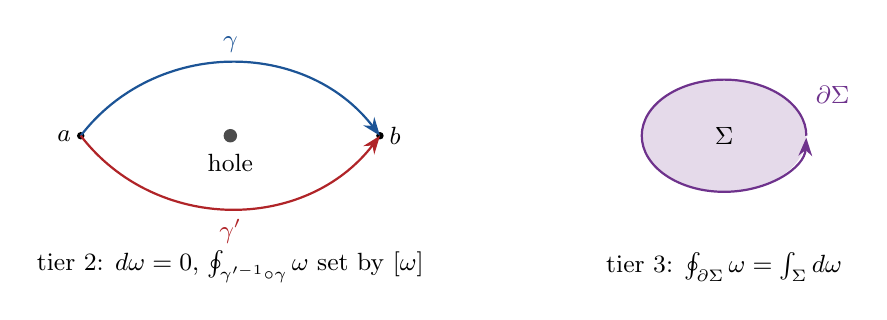
\begin{tikzpicture}[scale=0.95,>=Stealth]
\begin{scope}
\fill[black!70] (0,0) circle (0.09);
\node[below=3pt] at (0,0) {\small hole};
\fill (-2,0) circle (0.05) node[left] {\small $a$};
\fill (2,0) circle (0.05) node[right] {\small $b$};
\draw[accblue,thick,->] (-2,0) .. controls (-1,1.3) and (1,1.3) .. (2,0) node[pos=0.5,above] {\small $\gamma$};
\draw[ratered,thick,->] (-2,0) .. controls (-1,-1.3) and (1,-1.3) .. (2,0) node[pos=0.5,below] {\small $\gamma'$};
\node at (0,-1.75) {\small tier 2: $d\omega=0$, $\oint_{\gamma'^{-1}\circ\gamma}\omega$ set by $[\omega]$};
\end{scope}
\begin{scope}[xshift=6.6cm]
\fill[compurple!18] (0,0) ellipse (1.1 and 0.75);
\draw[compurple,thick,->] (1.1,0) arc (0:358:1.1 and 0.75);
\node at (0,0) {\small $\Sigma$};
\node[compurple] at (1.45,0.55) {\small $\partial\Sigma$};
\node at (0,-1.75) {\small tier 3: $\oint_{\partial\Sigma}\omega=\int_\Sigma d\omega$};
\end{scope}
\end{tikzpicture}
\end{center}

\noindent\textbf{Sketch 1: Gauss's law as an $H^2$ class.} On $\mathbb R^3\setminus\{0\}$ take $E=\hat r/r^2$. Then $\operatorname{div}E=0$ on the whole domain, and its flux form is
\begin{equation}
\star E^\flat=\sin\theta\,d\theta\wedge d\phi,\qquad d\star E^\flat=0,\qquad \oint_{S^2}\star E^\flat=4\pi\ne0.\tag{S1}\label{e:S1}
\end{equation}
Closed but not exact: $E$ is a curl on every contractible patch that misses the origin and on no neighbourhood of the whole sphere. Since $H^2_{\mathrm{dR}}(\mathbb R^3\setminus\{0\})\cong\mathbb R$, the enclosed charge is the coordinate of $[\star E^\flat]$. This is the precise answer to the question of Ref.~\cite{ghani}: zero divergence is the local condition, and the obstruction to a global potential is the sheaf-cohomology class.

\noindent\textbf{Sketch 2: conservation as closedness.} In four dimensions a current $j$ is conserved when
\begin{equation}
\nabla_\mu j^\mu=0\quad\Longleftrightarrow\quad d\star j^\flat=0,\tag{S2}\label{e:S2}
\end{equation}
and its charge through a closed hypersurface depends only on the homology class of that hypersurface, by Eq.~\eqref{e:8d} one degree up. For a symmetric rank-two tensor with $\nabla_\mu T^{\mu\nu}=0$ and a Killing field $\xi$,
\begin{equation}
j^\mu=T^{\mu\nu}\xi_\nu,\qquad \nabla_\mu j^\mu=(\nabla_\mu T^{\mu\nu})\xi_\nu+T^{\mu\nu}\nabla_{(\mu}\xi_{\nu)}=0,\tag{S3}\label{e:S3}
\end{equation}
so for Sec.~3.3 tensors that are conserved, $\nabla_\mu T^{\mu\nu}=0$, the charges are de Rham pairings of closed 3-forms. Sketch~3 supplies that condition in flat spacetime. For Markov processes, the correspondence between symmetries and conserved quantities is established as a Noether theorem~\cite{baezfong,gough}; Sketch~3 is the corresponding question for history-dependent accumulation.

\noindent\textbf{Sketch 3: accumulation preserves conservation in flat spacetime.} \Derived Take flat spacetime in Cartesian frames, trivial transports, $\Pi$ the identity on the symmetric slot pair, and a kernel depending only on proper time, as in Eq.~\eqref{e:59}. Writing $x'=x-y$, the causal past $J^-(x)$ becomes the fixed cone $y\in J^+(0)$, so the history term is a convolution,
\begin{equation}
T^{\mu\nu}(x)=\afrac\,J^{\mu\nu}(x)-(1-\afrac)\int_{J^+(0)}k\bigl(\tau(y)\bigr)\,J^{\mu\nu}(x-y)\,d^4y.\tag{S4}\label{e:S4}
\end{equation}
Where the integral and its derivative converge, $\partial_\mu$ passes inside with no boundary term from the light cone, since the domain no longer depends on $x$:
\begin{equation}
\partial_\mu T^{\mu\nu}=\afrac\,\partial_\mu J^{\mu\nu}-(1-\afrac)\,\bigl(k*\partial_\mu J^{\mu\nu}\bigr).\tag{S5}\label{e:S5}
\end{equation}
Hence a source conserved throughout the causal past yields a conserved accumulated tensor, for every $\afrac$. For the dyad profile $J^{\mu\nu}=x^\mu x^\nu$ with $x$ timelike, write $x^\mu=n\,u^\mu$ with $u\cdot u=1$; then $\partial_\mu J^{\mu\nu}=0$ is pressureless dust, $\partial_\mu(n^2u^\mu)=0$ together with $u^\mu\partial_\mu u^\nu=0$.

\noindent\textbf{Sketch 4: a cognitive-evolutionary hypothesis.} \Proposed Organisms that act on a physical world are selected for internal models that track the structure of that world. If physical dynamics is history-dependent with Markovian closure as a special case, as argued in Sec.~1, then neural dynamics that accumulate weighted history should be favored over purely instantaneous ones, at a metabolic cost below that of storing an expanding stack of past states. The hypothesis is that neural and cognitive memory should therefore show intermediate, power-law weighting of the kind given by Eq.~\eqref{e:20} for $0<\afrac<1$, and that judgment should show order dependence of the kind retained by the left closure in Eq.~\eqref{e:47}.

The available evidence supports both expectations. Retention in human memory follows power laws rather than exponentials~\cite{wixted}. Neocortical pyramidal neurons adapt on multiple timescales in a way that implements fractional-order differentiation of their input~\cite{lundstrom}. The vestibular system senses linear acceleration through the otoliths and angular motion through the semicircular canals; linear velocity is not sensed directly but obtained by integrating acceleration over time~\cite{angelaki}, so the velocity slot of the state $[x,v]$ is itself an accumulated quantity. Judgments depend on question order in a way that non-commuting projection models describe and classical probability models do not~\cite{wangqo,busemeyer}.

\noindent\textbf{Sketch 5: zero divisors, transport, and effective non-associativity.} \Derived The zero divisors of the carrier $M_2(\mathbb C)$ are its singular elements, $\det\sJ=0$. On the Hermitian slice, $\det X=0$ is exactly the null cone, so the zero divisors of the algebra meet the Hermitian slice exactly in the light cone: nonzero rank-one closures are null and rank-two closures are timelike (Sec.~3). Accumulation acts on this structure. The sum of two rank-one closures $\psi_1\psi_1^\dagger+\psi_2\psi_2^\dagger$ with $\psi_1,\psi_2$ linearly independent has rank two and positive determinant, so smearing null contributions from different directions of the causal past carries them into the interior of the cone. The accumulated carrier itself remains in the associative algebra $M_2(\mathbb C)$: Eq.~\eqref{e:9} is a linear weighted sum, and no step of it leaves $\mathbb C\otimes\mathbb H$.

\Proposed Products of carrier values at different events are another matter. To multiply $\sJ(q_1)$, $\sJ(q_2)$ and $\sJ(q_3)$ at a common event, each factor must first be transported. If the two bracketings route those transports along different paths, then for a flat connection the two results agree, and for a curved one they differ by the holonomy around the region the paths enclose, which appears as an associator of the transported product. The routing is part of the specification, not forced by the algebra.

\Derived An established instance is Jackiw's three-cocycle~\cite{jackiw}: translations in a magnetic field $B$ compose non-associatively exactly when $\nabla\cdot B\ne0$, with associator equal to the phase $e^{ie\Phi/\hbar}$, where $\Phi$ is the magnetic flux out of the tetrahedron spanned by the three translations. When $\nabla\cdot B=0$ everywhere the associator is trivial. For point monopoles, $B$ is closed on the punctured domain, the flux out of the tetrahedron pairs the $H^2$ class of Sketch~1 with the enclosed charge, and the associator is trivial exactly when the monopole charges satisfy the Dirac quantization condition.

\Proposed Transport smearing of the carrier spatializes its zero divisors and produces effective non-associativity of transported products, controlled by an $H^2$-type charge of the internal connection, one degree above the $H^1$ flux of Eq.~\eqref{e:54a}. Testing this requires the connection $\mathcal A_\mu$ to be specified: the test is to compute the associator of transported carrier products and compare it with the flux of the connection's curvature through the enclosed volume.

\noindent\textbf{Open.} In curved spacetime the propagators $P$ of Eq.~\eqref{e:9} and the soldering map of Sec.~3.3 enter, translation no longer maps $J^-(x)$ to a fixed cone, and $\nabla_\mu$ does not commute with the history integral; the commutator is curvature-dependent. Whether the history term preserves the closedness of Eq.~\eqref{e:S2}, and which charges in $H^3_{\mathrm{dR}}$ of a region it can carry, is a concrete test of the proposed dynamics.

\begin{symtab}{Sec.~7}
E & Point-charge field $\hat r/r^2$ (distinct from the bundle $E$) & vector field on $\mathbb R^3\setminus\{0\}$ & \eqref{e:S1}\\
j^\mu & Current & vector field & \eqref{e:S2}\\
\xi & Killing field & vector field & \eqref{e:S3}\\
y & Separation $x-x'$ & four-vector in $J^+(0)$ & \eqref{e:S4}\\
k*\cdot & Causal convolution with $k$ & linear operator & \eqref{e:S5}\\
n,\ u^\mu & Norm and unit direction of a timelike closure vector & positive real; four-velocity & Sec.~7\\
q_1,q_2,q_3 & Events at which carrier values are multiplied & spacetime points & Sec.~7\\
e,\ \Phi & Charge; magnetic flux out of a tetrahedron (distinct from $\Phi^a{}_b$) & real & Sec.~7\\
B & Magnetic field (distinct from $B(J,K)$) & vector field & Sec.~7\\
\end{symtab}




\begin{thebibliography}{99}\footnotesize\itemsep-0.8pt\setlength{\parskip}{0pt}
\bibitem{jackson} J.~D. Jackson, \textit{Classical Electrodynamics}, 3rd ed., Wiley (1999), Ch.~16.
\bibitem{maxey} M.~R. Maxey and J.~J. Riley, Equation of motion for a small rigid sphere in a nonuniform flow, \textit{Phys. Fluids} \textbf{26}, 883--889 (1983). doi:10.1063/1.864230
\bibitem{mashhoonsym} B.~Mashhoon, Nonlocal gravity: fundamental tetrads and constitutive relations, \textit{Symmetry} \textbf{14}, 2116 (2022). doi:10.3390/sym14102116. arXiv:2209.05817
\bibitem{mashhoon} B.~Mashhoon, \textit{Nonlocal Gravity}, International Series of Monographs on Physics 167, Oxford University Press (2017). doi:10.1093/oso/9780198803805.001.0001
\bibitem{woodard} R.~P. Woodard, Ostrogradsky's theorem on Hamiltonian instability, \textit{Scholarpedia} \textbf{10}, 32243 (2015). doi:10.4249/scholarpedia.32243. arXiv:1506.02210
\bibitem{rosicky} J.~Rosick\'y, Abstract tangent functors, \textit{Diagrammes} \textbf{12}, Expos\'e 3, JR1--JR11 (1984).
\bibitem{cockett2014} J.~R.~B. Cockett and G.~S.~H. Cruttwell, Differential structure, tangent structure, and SDG, \textit{Appl. Categ. Structures} \textbf{22}, 331--417 (2014). doi:10.1007/s10485-013-9312-0
\bibitem{cockett2017} J.~R.~B. Cockett and G.~S.~H. Cruttwell, Connections in tangent categories, \textit{Theory Appl. Categ.} \textbf{32}, No.~26, 835--888 (2017).
\bibitem{pavlovic} D.~Pavlovi\'c and M.~H. Escard\'o, Calculus in coinductive form, \textit{Proc. 13th IEEE Symposium on Logic in Computer Science (LICS)}, 408--417 (1998). doi:10.1109/LICS.1998.705675
\bibitem{rutten} J.~J.~M.~M. Rutten, Behavioural differential equations: a coinductive calculus of streams, automata, and power series, \textit{Theoret. Comput. Sci.} \textbf{308}, 1--53 (2003). doi:10.1016/S0304-3975(02)00895-2
\bibitem{caldirola} P.~Caldirola, Forze non conservative nella meccanica quantistica, \textit{Nuovo Cimento} \textbf{18}, 393--400 (1941). doi:10.1007/BF02960144
\bibitem{kanai} E.~Kanai, On the quantization of the dissipative systems, \textit{Prog. Theor. Phys.} \textbf{3}, 440--442 (1948). doi:10.1143/ptp/3.4.440
\bibitem{weinbergcosmo} S.~Weinberg, \textit{Cosmology}, Oxford University Press (2008).
\bibitem{furey} C.~Furey, \textit{Standard Model Physics from an Algebra?}, PhD thesis, University of Waterloo (2015), Ch.~3. arXiv:1611.09182
\bibitem{baez} J.~C. Baez, The octonions, \textit{Bull. Amer. Math. Soc.} \textbf{39}, 145--205 (2002). doi:10.1090/S0273-0979-01-00934-X. arXiv:math/0105155
\bibitem{baezhuertasusy} J.~C. Baez and J.~Huerta, Division algebras and supersymmetry I, in \textit{Superstrings, Geometry, Topology, and C*-algebras}, Proc. Symp. Pure Math. \textbf{81}, AMS (2010), pp.~65--80. doi:10.1090/pspum/081/2681758. arXiv:0909.0551
\bibitem{feynman} R.~P. Feynman, Space-time approach to non-relativistic quantum mechanics, \textit{Rev. Mod. Phys.} \textbf{20}, 367--387 (1948). doi:10.1103/RevModPhys.20.367
\bibitem{quantropy} J.~C. Baez and B.~S. Pollard, Quantropy, \textit{Entropy} \textbf{17}, 772--789 (2015). doi:10.3390/e17020772. arXiv:1311.0813
\bibitem{browngray} R.~B. Brown and A.~Gray, Vector cross products, \textit{Comment. Math. Helv.} \textbf{42}, 222--236 (1967). doi:10.1007/BF02564418
\bibitem{riesz} M.~Riesz, L'int\'egrale de Riemann--Liouville et le probl\`eme de Cauchy, \textit{Acta Math.} \textbf{81}, 1--222 (1949). doi:10.1007/BF02395016
\bibitem{samko} S.~G. Samko, A.~A. Kilbas, and O.~I. Marichev, \textit{Fractional Integrals and Derivatives: Theory and Applications}, Gordon and Breach (1993).
\bibitem{podlubny} I.~Podlubny, \textit{Fractional Differential Equations}, Mathematics in Science and Engineering 198, Academic Press (1999).
\bibitem{mori} H.~Mori, Transport, collective motion, and Brownian motion, \textit{Prog. Theor. Phys.} \textbf{33}, 423--455 (1965). doi:10.1143/PTP.33.423
\bibitem{zwanzig} R.~Zwanzig, \textit{Nonequilibrium Statistical Mechanics}, Oxford University Press (2001).
\bibitem{wixted} J.~T. Wixted and E.~B. Ebbesen, On the form of forgetting, \textit{Psychol. Sci.} \textbf{2}, 409--415 (1991). doi:10.1111/j.1467-9280.1991.tb00175.x
\bibitem{lundstrom} B.~N. Lundstrom, M.~H. Higgs, W.~J. Spain, and A.~L. Fairhall, Fractional differentiation by neocortical pyramidal neurons, \textit{Nat. Neurosci.} \textbf{11}, 1335--1342 (2008). doi:10.1038/nn.2212
\bibitem{angelaki} D.~E. Angelaki and K.~E. Cullen, Vestibular system: the many facets of a multimodal sense, \textit{Annu. Rev. Neurosci.} \textbf{31}, 125--150 (2008). doi:10.1146/annurev.neuro.31.060407.125555
\bibitem{wangqo} Z.~Wang, T.~Solloway, R.~M. Shiffrin, and J.~R. Busemeyer, Context effects produced by question orders reveal quantum nature of human judgments, \textit{Proc. Natl. Acad. Sci. USA} \textbf{111}, 9431--9436 (2014). doi:10.1073/pnas.1407756111
\bibitem{busemeyer} J.~R. Busemeyer and P.~D. Bruza, \textit{Quantum Models of Cognition and Decision}, Cambridge University Press (2012).
\bibitem{landauer} R.~Landauer, Irreversibility and heat generation in the computing process, \textit{IBM J. Res. Dev.} \textbf{5}, 183--191 (1961). doi:10.1147/rd.53.0183
\bibitem{bekenstein1981} J.~D. Bekenstein, Universal upper bound on the entropy-to-energy ratio for bounded systems, \textit{Phys. Rev. D} \textbf{23}, 287--298 (1981). doi:10.1103/PhysRevD.23.287
\bibitem{bankssusskindpeskin} T.~Banks, L.~Susskind, and M.~E. Peskin, Difficulties for the evolution of pure states into mixed states, \textit{Nucl. Phys. B} \textbf{244}, 125--134 (1984). doi:10.1016/0550-3213(84)90184-6
\bibitem{bennett2003} C.~H. Bennett, Notes on Landauer's principle, reversible computation, and Maxwell's demon, \textit{Stud. Hist. Phil. Mod. Phys.} \textbf{34}, 501--510 (2003). doi:10.1016/S1355-2198(03)00039-X. arXiv:physics/0210005
\bibitem{jackiw} R.~Jackiw, Three-cocycle in mathematics and physics, \textit{Phys. Rev. Lett.} \textbf{54}, 159--162 (1985). doi:10.1103/PhysRevLett.54.159
\bibitem{pearl} J.~Pearl, \textit{Causality: Models, Reasoning, and Inference}, 2nd ed., Cambridge University Press (2009).
\bibitem{vaswani} A.~Vaswani, N.~Shazeer, N.~Parmar, J.~Uszkoreit, L.~Jones, A.~N. Gomez, {\L}.~Kaiser, and I.~Polosukhin, Attention is all you need, \textit{Advances in Neural Information Processing Systems} \textbf{30} (2017). arXiv:1706.03762
\bibitem{maynardsmith} J.~Maynard Smith, \textit{Evolution and the Theory of Games}, Cambridge University Press (1982).
\bibitem{baezpollardre} J.~C. Baez and B.~S. Pollard, Relative entropy in biological systems, \textit{Entropy} \textbf{18}, 46 (2016). doi:10.3390/e18020046. arXiv:1512.02742
\bibitem{hofbauer} J.~Hofbauer and K.~Sigmund, \textit{Evolutionary Games and Population Dynamics}, Cambridge University Press (1998).
\bibitem{baezbio} J.~C. Baez, Biology as information dynamics, lecture slides (2017), \texttt{math.ucr.edu/home/baez/bio\_asu}.
\bibitem{harper} M.~Harper, Information geometry and evolutionary game theory, arXiv:0911.1383 (2009).
\bibitem{baezbiamonte} J.~C. Baez and J.~D. Biamonte, \textit{Quantum Techniques in Stochastic Mechanics}, World Scientific (2018). arXiv:1209.3632
\bibitem{doi} M.~Doi, Second quantization representation for classical many-particle system, \textit{J. Phys. A} \textbf{9}, 1465--1477 (1976). doi:10.1088/0305-4470/9/9/008
\bibitem{baezfongpollard} J.~C. Baez, B.~Fong, and B.~S. Pollard, A compositional framework for Markov processes, \textit{J. Math. Phys.} \textbf{57}, 033301 (2016). doi:10.1063/1.4941578
\bibitem{fongspivak} B.~Fong and D.~I. Spivak, \textit{An Invitation to Applied Category Theory: Seven Sketches in Compositionality}, Cambridge University Press (2019). arXiv:1803.05316
\bibitem{baezstay} J.~C. Baez and M.~Stay, Physics, topology, logic and computation: a Rosetta Stone, in B.~Coecke (ed.), \textit{New Structures for Physics}, Lecture Notes in Physics \textbf{813}, Springer (2011), pp.~95--172. doi:10.1007/978-3-642-12821-9\_2. arXiv:0903.0340
\bibitem{baezpollardrn} J.~C. Baez and B.~S. Pollard, A compositional framework for reaction networks, \textit{Rev. Math. Phys.} \textbf{29}, 1750028 (2017). doi:10.1142/S0129055X17500283
\bibitem{hornjackson} F.~Horn and R.~Jackson, General mass action kinetics, \textit{Arch. Rational Mech. Anal.} \textbf{47}, 81--116 (1972). doi:10.1007/BF00251225
\bibitem{baezfong} J.~C. Baez and B.~Fong, A Noether theorem for Markov processes, \textit{J. Math. Phys.} \textbf{54}, 013301 (2013). doi:10.1063/1.4773921
\bibitem{gough} J.~E. Gough, T.~S. Ratiu, and O.~G. Smolyanov, Noether's theorem for dissipative quantum dynamical semi-groups, \textit{J. Math. Phys.} \textbf{56}, 022108 (2015). doi:10.1063/1.4907985
\bibitem{baylis} W.~E. Baylis, Special relativity with $2\times2$ matrices, \textit{Am. J. Phys.} \textbf{48}, 918--925 (1980). doi:10.1119/1.12202
\bibitem{penrose} R.~Penrose and W.~Rindler, \textit{Spinors and Space-Time, Vol.~1: Two-Spinor Calculus and Relativistic Fields}, Cambridge University Press (1984).
\bibitem{penrosetwistor} R.~Penrose, Twistor algebra, \textit{J. Math. Phys.} \textbf{8}, 345--366 (1967). doi:10.1063/1.1705200
\bibitem{samuel} J.~Samuel, K.~Shivam, and S.~Sinha, Lorentzian geometry for detecting qubit entanglement, \textit{Ann. Phys.} \textbf{396}, 159--172 (2018). doi:10.1016/j.aop.2018.07.019. arXiv:1801.00611
\bibitem{verstraete} F.~Verstraete, J.~Dehaene, and B.~De Moor, Local filtering operations on two qubits, \textit{Phys. Rev. A} \textbf{64}, 010101(R) (2001), doi:10.1103/PhysRevA.64.010101; Lorentz singular-value decomposition and its applications to pure states of three qubits, \textit{Phys. Rev. A} \textbf{65}, 032308 (2002), doi:10.1103/PhysRevA.65.032308.
\bibitem{fulton} W.~Fulton and J.~Harris, \textit{Representation Theory: A First Course}, Graduate Texts in Mathematics 129, Springer (1991).
\bibitem{nappi} C.~R. Nappi and E.~Witten, Wess--Zumino--Witten model based on a nonsemisimple group, \textit{Phys. Rev. Lett.} \textbf{71}, 3751--3753 (1993). doi:10.1103/PhysRevLett.71.3751. arXiv:hep-th/9310112
\bibitem{weinberg} S.~Weinberg, \textit{The Quantum Theory of Fields, Vol.~2: Modern Applications}, Cambridge University Press (1996), Sec.~15.2.
\bibitem{gellmann} S.~L. Glashow and M.~Gell-Mann, Gauge theories of vector particles, \textit{Ann. Phys. (N.Y.)} \textbf{15}, 437--460 (1961). doi:10.1016/0003-4916(61)90193-2
\bibitem{derdzinski} A.~Derdzinski and \'S.~R. Gal, Indefinite Einstein metrics on simple Lie groups, \textit{Indiana Univ. Math. J.} \textbf{63}, 165--212 (2014), Sec.~13. doi:10.1512/iumj.2014.63.5191. arXiv:1209.6084
\bibitem{wilson} K.~G. Wilson, Confinement of quarks, \textit{Phys. Rev. D} \textbf{10}, 2445--2459 (1974). doi:10.1103/PhysRevD.10.2445
\bibitem{roiesnel} C.~Roiesnel, On the U(2) lattice gauge theory, arXiv:hep-lat/9509092 (1995).
\bibitem{ab} Y.~Aharonov and D.~Bohm, Significance of electromagnetic potentials in the quantum theory, \textit{Phys. Rev.} \textbf{115}, 485--491 (1959). doi:10.1103/PhysRev.115.485
\bibitem{wuyang} T.~T. Wu and C.~N. Yang, Concept of nonintegrable phase factors and global formulation of gauge fields, \textit{Phys. Rev. D} \textbf{12}, 3845--3857 (1975). doi:10.1103/PhysRevD.12.3845
\bibitem{baezhuerta} J.~C. Baez and J.~Huerta, An invitation to higher gauge theory, \textit{Gen. Relativ. Gravit.} \textbf{43}, 2335--2392 (2011). doi:10.1007/s10714-010-1070-9. arXiv:1003.4485
\bibitem{urbantke} H.~Urbantke, On integrability properties of SU(2) Yang--Mills fields. I. Infinitesimal part, \textit{J. Math. Phys.} \textbf{25}, 2321--2324 (1984). doi:10.1063/1.526402
\bibitem{plebanski} J.~F. Pleba\'nski, On the separation of Einsteinian substructures, \textit{J. Math. Phys.} \textbf{18}, 2511--2520 (1977). doi:10.1063/1.523215
\bibitem{cdj} R.~Capovilla, T.~Jacobson, and J.~Dell, General relativity without the metric, \textit{Phys. Rev. Lett.} \textbf{63}, 2325--2328 (1989). doi:10.1103/PhysRevLett.63.2325
\bibitem{krasnov} K.~Krasnov, Pure connection action principle for general relativity, \textit{Phys. Rev. Lett.} \textbf{106}, 251103 (2011). doi:10.1103/PhysRevLett.106.251103. arXiv:1103.4498
\bibitem{freidel} L.~Freidel, Modified gravity without new degrees of freedom, arXiv:0812.3200 (2008).
\bibitem{baezspinfoam} J.~C. Baez, Spin foam models, \textit{Class. Quantum Grav.} \textbf{15}, 1827--1858 (1998). doi:10.1088/0264-9381/15/7/004. arXiv:gr-qc/9709052
\bibitem{bombelli} L.~Bombelli, J.~Lee, D.~Meyer, and R.~D. Sorkin, Space-time as a causal set, \textit{Phys. Rev. Lett.} \textbf{59}, 521--524 (1987). doi:10.1103/PhysRevLett.59.521
\bibitem{botttu} R.~Bott and L.~W. Tu, \textit{Differential Forms in Algebraic Topology}, Graduate Texts in Mathematics 82, Springer (1982).
\bibitem{hatcher} A.~Hatcher, \textit{Algebraic Topology}, Cambridge University Press (2002), Sec.~3.1.
\bibitem{ghani} N.~Ghani, private communication (October 2026).
\bibitem{jarlskog} C.~Jarlskog, Commutator of the quark mass matrices in the standard electroweak model and a measure of maximal CP nonconservation, \textit{Phys. Rev. Lett.} \textbf{55}, 1039--1042 (1985). doi:10.1103/PhysRevLett.55.1039
\end{thebibliography}

\end{document}
